\documentclass[twoside]{book}

% Packages required by doxygen
\usepackage{fixltx2e}
\usepackage{calc}
\usepackage{doxygen}
\usepackage[export]{adjustbox} % also loads graphicx
\usepackage{graphicx}
\usepackage[utf8]{inputenc}
\usepackage{makeidx}
\usepackage{multicol}
\usepackage{multirow}
\PassOptionsToPackage{warn}{textcomp}
\usepackage{textcomp}
\usepackage[nointegrals]{wasysym}
\usepackage[table]{xcolor}

% Font selection
\usepackage[T1]{fontenc}
\usepackage[scaled=.90]{helvet}
\usepackage{courier}
\usepackage{amssymb}
\usepackage{sectsty}
\renewcommand{\familydefault}{\sfdefault}
\allsectionsfont{%
  \fontseries{bc}\selectfont%
  \color{darkgray}%
}
\renewcommand{\DoxyLabelFont}{%
  \fontseries{bc}\selectfont%
  \color{darkgray}%
}
\newcommand{\+}{\discretionary{\mbox{\scriptsize$\hookleftarrow$}}{}{}}

% Page & text layout
\usepackage{geometry}
\geometry{%
  a4paper,%
  top=2.5cm,%
  bottom=2.5cm,%
  left=2.5cm,%
  right=2.5cm%
}
\tolerance=750
\hfuzz=15pt
\hbadness=750
\setlength{\emergencystretch}{15pt}
\setlength{\parindent}{0cm}
\setlength{\parskip}{3ex plus 2ex minus 2ex}
\makeatletter
\renewcommand{\paragraph}{%
  \@startsection{paragraph}{4}{0ex}{-1.0ex}{1.0ex}{%
    \normalfont\normalsize\bfseries\SS@parafont%
  }%
}
\renewcommand{\subparagraph}{%
  \@startsection{subparagraph}{5}{0ex}{-1.0ex}{1.0ex}{%
    \normalfont\normalsize\bfseries\SS@subparafont%
  }%
}
\makeatother

% Headers & footers
\usepackage{fancyhdr}
\pagestyle{fancyplain}
\fancyhead[LE]{\fancyplain{}{\bfseries\thepage}}
\fancyhead[CE]{\fancyplain{}{}}
\fancyhead[RE]{\fancyplain{}{\bfseries\leftmark}}
\fancyhead[LO]{\fancyplain{}{\bfseries\rightmark}}
\fancyhead[CO]{\fancyplain{}{}}
\fancyhead[RO]{\fancyplain{}{\bfseries\thepage}}
\fancyfoot[LE]{\fancyplain{}{}}
\fancyfoot[CE]{\fancyplain{}{}}
\fancyfoot[RE]{\fancyplain{}{\bfseries\scriptsize Generated by Doxygen }}
\fancyfoot[LO]{\fancyplain{}{\bfseries\scriptsize Generated by Doxygen }}
\fancyfoot[CO]{\fancyplain{}{}}
\fancyfoot[RO]{\fancyplain{}{}}
\renewcommand{\footrulewidth}{0.4pt}
\renewcommand{\chaptermark}[1]{%
  \markboth{#1}{}%
}
\renewcommand{\sectionmark}[1]{%
  \markright{\thesection\ #1}%
}

% Indices & bibliography
\usepackage{natbib}
\usepackage[titles]{tocloft}
\setcounter{tocdepth}{3}
\setcounter{secnumdepth}{5}
\makeindex

% Hyperlinks (required, but should be loaded last)
\usepackage{ifpdf}
\ifpdf
  \usepackage[pdftex,pagebackref=true]{hyperref}
\else
  \usepackage[ps2pdf,pagebackref=true]{hyperref}
\fi
\hypersetup{%
  colorlinks=true,%
  linkcolor=blue,%
  citecolor=blue,%
  unicode%
}

% Custom commands
\newcommand{\clearemptydoublepage}{%
  \newpage{\pagestyle{empty}\cleardoublepage}%
}

\usepackage{caption}
\captionsetup{labelsep=space,justification=centering,font={bf},singlelinecheck=off,skip=4pt,position=top}

%===== C O N T E N T S =====

\begin{document}

% Titlepage & ToC
\hypersetup{pageanchor=false,
             bookmarksnumbered=true,
             pdfencoding=unicode
            }
\pagenumbering{alph}
\begin{titlepage}
\vspace*{7cm}
\begin{center}%
{\Large pr\+S63\+Brute\+Force }\\
\vspace*{1cm}
{\large Generated by Doxygen 1.8.13}\\
\end{center}
\end{titlepage}
\clearemptydoublepage
\pagenumbering{roman}
\tableofcontents
\clearemptydoublepage
\pagenumbering{arabic}
\hypersetup{pageanchor=true}

%--- Begin generated contents ---
\chapter{Проект показывающий стиль написания ПО}
\label{index}\hypertarget{index}{}\begin{DoxyAuthor}{Author}
Антонов А.\+Л +7(958)201.\+5452 
\end{DoxyAuthor}

\chapter{Описание алгоритма работы клиента для распределённой системы подбора пароля по раскдированию файлов защищённых по схеме S63}
\label{md__home_antonov_work_project_pr_s63_brute_force_client_pr_s63_brute_force_client_readme}
\Hypertarget{md__home_antonov_work_project_pr_s63_brute_force_client_pr_s63_brute_force_client_readme}

\begin{DoxyEnumerate}
\item При запуске клиент выполняет поиск сервера или этот поиск может быть выполнен вручную.
\item Если сервер найден, то клиент запрашивает сервер о подключении (connection\+Request);
\item Сервер подтверждает подключение (connection\+Confirm) и передает клиенту размер блока для подбора ключей и первые 8 байт которые нужно расшифровывать;
\item Получив подтверждение клиент переходит в режим ожидания команд от сервера;
\item Раз в фиксированный промежуток времени клиент проверяет подключенность к серверу (state\+Request). Если за этот промежуток времени уже было подключение к серверу для передачи данных, то запрос не выполняется, а время ожидания начинается после завершения обмена данными.
\item Находясь в режиме ожидания, клиент получает от сервера начальный ключ блока данных (transfer\+Data).
\item Клиент подтверждает (accept\+Data) или отказывается (refuse\+Data) от приема данных. При отказе, сервер запрашивает состояние клиента и если клиент находится в режиме ожидания, то через определённый промежуток времени повторяет передачу начального ключа, при этом ключ может отличааться от первоначального.
\item Получив ключ выполняет подбор пароля для первых 8 байт и если в результате дешиврации получается начальная сигнатура zip-\/файла, то передает этот ключ серверу (transfer\+Data). Сервер подтверждает (accept\+Data) получения ключа. При отказе (refuse\+Data) клиент через определенный промежуток времени повторяет передачу данных до тех пол, пока данные не будут приняты сервером. Если в результате подбора полученно несколько ключей, то они передаются последовательно;
\item После проверки всех ключей блока, клиент запрашивает новый блок ключей (transfer\+Request) и либо получает его или переходит в режим ожидания.
\item В любой момент может быть получен запрос состояния от сервера (state\+Request). В ответ на этот запрос клиент возвращает своё состояние (state\+Confirm).
\item Соединение между клиентом и сервером открывается при нахождении сервера и т.\+к. предполагается, что большого количествава клиентов не будет, то остается постоянно открытым. 
\end{DoxyEnumerate}
\chapter{L\+I\+C\+E\+N\+SE}
\label{md__home_antonov_work_project_pr_s63_brute_force__l_i_c_e_n_s_e}
\Hypertarget{md__home_antonov_work_project_pr_s63_brute_force__l_i_c_e_n_s_e}
The M\+IT License (M\+IT)

Copyright (c) 2019

Permission is hereby granted, free of charge, to any person obtaining a copy of this software and associated documentation files (the \char`\"{}\+Software\char`\"{}), to deal in the Software without restriction, including without limitation the rights to use, copy, modify, merge, publish, distribute, sublicense, and/or sell copies of the Software, and to permit persons to whom the Software is furnished to do so, subject to the following conditions\+:

The above copyright notice and this permission notice shall be included in all copies or substantial portions of the Software.

T\+HE S\+O\+F\+T\+W\+A\+RE IS P\+R\+O\+V\+I\+D\+ED \char`\"{}\+A\+S I\+S\char`\"{}, W\+I\+T\+H\+O\+UT W\+A\+R\+R\+A\+N\+TY OF A\+NY K\+I\+ND, E\+X\+P\+R\+E\+SS OR I\+M\+P\+L\+I\+ED, I\+N\+C\+L\+U\+D\+I\+NG B\+UT N\+OT L\+I\+M\+I\+T\+ED TO T\+HE W\+A\+R\+R\+A\+N\+T\+I\+ES OF M\+E\+R\+C\+H\+A\+N\+T\+A\+B\+I\+L\+I\+TY, F\+I\+T\+N\+E\+SS F\+OR A P\+A\+R\+T\+I\+C\+U\+L\+AR P\+U\+R\+P\+O\+SE A\+ND N\+O\+N\+I\+N\+F\+R\+I\+N\+G\+E\+M\+E\+NT. IN NO E\+V\+E\+NT S\+H\+A\+LL T\+HE A\+U\+T\+H\+O\+RS OR C\+O\+P\+Y\+R\+I\+G\+HT H\+O\+L\+D\+E\+RS BE L\+I\+A\+B\+LE F\+OR A\+NY C\+L\+A\+IM, D\+A\+M\+A\+G\+ES OR O\+T\+H\+ER L\+I\+A\+B\+I\+L\+I\+TY, W\+H\+E\+T\+H\+ER IN AN A\+C\+T\+I\+ON OF C\+O\+N\+T\+R\+A\+CT, T\+O\+RT OR O\+T\+H\+E\+R\+W\+I\+SE, A\+R\+I\+S\+I\+NG F\+R\+OM, O\+UT OF OR IN C\+O\+N\+N\+E\+C\+T\+I\+ON W\+I\+TH T\+HE S\+O\+F\+T\+W\+A\+RE OR T\+HE U\+SE OR O\+T\+H\+ER D\+E\+A\+L\+I\+N\+GS IN T\+HE S\+O\+F\+T\+W\+A\+RE. 
\chapter{Пример демонстрирующий работу распределенной по локальной сети системы подбора пароля для файлов с морскими картами защищенными по схеме S63 (данный пример пока находится в стадии разработки)}
\label{md__home_antonov_work_project_pr_s63_brute_force__r_e_a_d_m_e}
\Hypertarget{md__home_antonov_work_project_pr_s63_brute_force__r_e_a_d_m_e}
\subsection*{Описание примера\+:}


\begin{DoxyItemize}
\item В сети есть сервер к которому подключаются клиенты.
\item Сервер не только распределяет блоки ключей выдаваемые клиентам, но и сам выступает в качестве клиента.
\item После запуска клиенты сами выполняют поиск сервера. Для этого номер порта должен быть уникальный в ЛВС или адрес и порт можно ввести вручную.
\item Клиенты выполняют подбор ключа для первых 8ми байтам файла зашифрованного по алгоритму Blowfish и если на выходе получается число 0x04034b50, то этот ключ передается серверу для окончательной проверки и дешифрации всего файла.
\item Если проверка прошла успешно, то всем остальным клиентам передается команда на прекращение подбора.
\end{DoxyItemize}

\subsection*{В данном примере показаны\+:}


\begin{DoxyItemize}
\item Знания с++11;
\item ООП;
\item Создание кросплатформенных приложений (Debian Linux, Astra Linux SE 1.\+6, Window 10 (7);
\item Работа с многопоточностью (std\+::thread);
\item Работа приложений по принципу клиент-\/сервер (Qt\+Network, Q\+Tcp\+Server, Q\+Tcp\+Socket и т.\+д.);
\item Работа с системами шифрирования данных (библиотека Botan);
\item Создание пользовательских интерфейсов;
\item Создание библиотек и кросплатформенная работа с ними;
\item Создание Unit test для приложения;
\item Умение работать с документацией на английском языке (Изучено описание схемы защмты данных для морских карт S63 и описание протокола передачи данных S57 www.\+iho.\+int и библиотеки Botan \href{https://botan.randombit.net}{\tt https\+://botan.\+randombit.\+net}).
\item В дальнейшем планируется использование на транспортном уровне T\+LS (библиотека Botan).
\end{DoxyItemize}

Вся документация к проекту и создаваемым классам выполнена по стандарту doxygen. 
\chapter{Hierarchical Index}
\section{Class Hierarchy}
This inheritance list is sorted roughly, but not completely, alphabetically\+:\begin{DoxyCompactList}
\item \contentsline{section}{server\+:\+:common\+Define\+Server\+:\+:brut\+Force\+Item}{\pageref{structserver_1_1common_define_server_1_1brut_force_item}}{}
\item \contentsline{section}{server\+:\+:common\+Define\+Server\+:\+:client\+Descr}{\pageref{structserver_1_1common_define_server_1_1client_descr}}{}
\item error\+\_\+category\begin{DoxyCompactList}
\item \contentsline{section}{blowfish\+Lib\+:\+:blowfish\+Exeption\+:\+:T\+Blowfish\+Exeption\+Category}{\pageref{structblowfish_lib_1_1blowfish_exeption_1_1_t_blowfish_exeption_category}}{}
\item \contentsline{section}{exception\+:\+:T\+Exception\+Category}{\pageref{classexception_1_1_t_exception_category}}{}
\end{DoxyCompactList}
\item exception\begin{DoxyCompactList}
\item \contentsline{section}{blowfish\+Lib\+:\+:blowfish\+Exeption\+:\+:T\+Blowfish\+Exeption}{\pageref{classblowfish_lib_1_1blowfish_exeption_1_1_t_blowfish_exeption}}{}
\item \contentsline{section}{exception\+:\+:T\+Exception}{\pageref{classexception_1_1_t_exception}}{}
\end{DoxyCompactList}
\item \contentsline{section}{blowfish\+Lib\+:\+:Local\+File\+Header}{\pageref{structblowfish_lib_1_1_local_file_header}}{}
\item \contentsline{section}{server\+:\+:common\+Define\+Server\+:\+:log\+Item}{\pageref{structserver_1_1common_define_server_1_1log_item}}{}
\item Q\+Abstract\+Table\+Model\begin{DoxyCompactList}
\item \contentsline{section}{client\+:\+:T\+Client\+Model}{\pageref{classclient_1_1_t_client_model}}{}
\item \contentsline{section}{T\+Server\+Log\+Model}{\pageref{class_t_server_log_model}}{}
\end{DoxyCompactList}
\item Q\+Main\+Window\begin{DoxyCompactList}
\item \contentsline{section}{client\+:\+:pr\+S63\+Brute\+Force\+Client}{\pageref{classclient_1_1pr_s63_brute_force_client}}{}
\item \contentsline{section}{server\+:\+:pr\+S63\+Brute\+Force\+Server}{\pageref{classserver_1_1pr_s63_brute_force_server}}{}
\end{DoxyCompactList}
\item Q\+Object\begin{DoxyCompactList}
\item \contentsline{section}{connection\+:\+:T\+Connection}{\pageref{classconnection_1_1_t_connection}}{}
\begin{DoxyCompactList}
\item \contentsline{section}{connection\+:\+:T\+Connection\+Client}{\pageref{classconnection_1_1_t_connection_client}}{}
\item \contentsline{section}{connection\+:\+:T\+Connection\+Server}{\pageref{classconnection_1_1_t_connection_server}}{}
\begin{DoxyCompactList}
\item \contentsline{section}{server\+:\+:T\+Brute\+Force\+Manager}{\pageref{classserver_1_1_t_brute_force_manager}}{}
\end{DoxyCompactList}
\end{DoxyCompactList}
\end{DoxyCompactList}
\item \contentsline{section}{blowfish\+Lib\+:\+:T\+Blowfish}{\pageref{classblowfish_lib_1_1_t_blowfish}}{}
\item \contentsline{section}{connection\+:\+:T\+Data\+Transfer}{\pageref{structconnection_1_1_t_data_transfer}}{}
\item \contentsline{section}{common\+Define\+Client\+:\+:T\+Log\+Item\+Client}{\pageref{structcommon_define_client_1_1_t_log_item_client}}{}
\item vector\begin{DoxyCompactList}
\item \contentsline{section}{client\+:\+:T\+Client\+Model}{\pageref{classclient_1_1_t_client_model}}{}
\item \contentsline{section}{T\+Server\+Log\+Model}{\pageref{class_t_server_log_model}}{}
\end{DoxyCompactList}
\end{DoxyCompactList}

\chapter{Class Index}
\section{Class List}
Here are the classes, structs, unions and interfaces with brief descriptions\+:\begin{DoxyCompactList}
\item\contentsline{section}{\hyperlink{structserver_1_1common_define_server_1_1brut_force_item}{server\+::common\+Define\+Server\+::brut\+Force\+Item} \\*Структура данных для одной итерации подбора }{\pageref{structserver_1_1common_define_server_1_1brut_force_item}}{}
\item\contentsline{section}{\hyperlink{structblowfish_lib_1_1_local_file_header}{blowfish\+Lib\+::\+Local\+File\+Header} \\*Описание метаданных работы с Z\+IP }{\pageref{structblowfish_lib_1_1_local_file_header}}{}
\item\contentsline{section}{\hyperlink{classclient_1_1pr_s63_brute_force_client}{client\+::pr\+S63\+Brute\+Force\+Client} \\*Форма главного окна клиента для подбора пароля }{\pageref{classclient_1_1pr_s63_brute_force_client}}{}
\item\contentsline{section}{\hyperlink{classserver_1_1pr_s63_brute_force_server}{server\+::pr\+S63\+Brute\+Force\+Server} }{\pageref{classserver_1_1pr_s63_brute_force_server}}{}
\item\contentsline{section}{\hyperlink{classblowfish_lib_1_1_t_blowfish}{blowfish\+Lib\+::\+T\+Blowfish} \\*Класс выполняющий декодирование S63 и запись файла S57 }{\pageref{classblowfish_lib_1_1_t_blowfish}}{}
\item\contentsline{section}{\hyperlink{classblowfish_lib_1_1blowfish_exeption_1_1_t_blowfish_exeption}{blowfish\+Lib\+::blowfish\+Exeption\+::\+T\+Blowfish\+Exeption} \\*Класс обработки ошибок при декодировании }{\pageref{classblowfish_lib_1_1blowfish_exeption_1_1_t_blowfish_exeption}}{}
\item\contentsline{section}{\hyperlink{structblowfish_lib_1_1blowfish_exeption_1_1_t_blowfish_exeption_category}{blowfish\+Lib\+::blowfish\+Exeption\+::\+T\+Blowfish\+Exeption\+Category} \\*Структура для формирования std\+::error\+\_\+code для класса декодирования }{\pageref{structblowfish_lib_1_1blowfish_exeption_1_1_t_blowfish_exeption_category}}{}
\item\contentsline{section}{\hyperlink{classserver_1_1_t_brute_force_manager}{server\+::\+T\+Brute\+Force\+Manager} \\*Класс выполняющий управление и распределение блоков между клиентами (в том числе локальным) }{\pageref{classserver_1_1_t_brute_force_manager}}{}
\item\contentsline{section}{\hyperlink{classclient_1_1_t_client_model}{client\+::\+T\+Client\+Model} \\*Модель для отображения лога работы клиента }{\pageref{classclient_1_1_t_client_model}}{}
\item\contentsline{section}{\hyperlink{classconnection_1_1_t_connection}{connection\+::\+T\+Connection} \\*Базовый класс для обслуживания работы распределенной системы }{\pageref{classconnection_1_1_t_connection}}{}
\item\contentsline{section}{\hyperlink{classconnection_1_1_t_connection_client}{connection\+::\+T\+Connection\+Client} \\*Класс для работы с сервером раздающим блоки ключей для подбора }{\pageref{classconnection_1_1_t_connection_client}}{}
\item\contentsline{section}{\hyperlink{classconnection_1_1_t_connection_server}{connection\+::\+T\+Connection\+Server} \\*Класс для работы с распределённой системой подбора ключей }{\pageref{classconnection_1_1_t_connection_server}}{}
\item\contentsline{section}{\hyperlink{structconnection_1_1_t_data_transfer}{connection\+::\+T\+Data\+Transfer} \\*The \hyperlink{structconnection_1_1_t_data_transfer}{T\+Data\+Transfer} struct Формат передаваемых данных }{\pageref{structconnection_1_1_t_data_transfer}}{}
\item\contentsline{section}{\hyperlink{classexception_1_1_t_exception}{exception\+::\+T\+Exception} \\*Класс обработки ошибок }{\pageref{classexception_1_1_t_exception}}{}
\item\contentsline{section}{\hyperlink{classexception_1_1_t_exception_category}{exception\+::\+T\+Exception\+Category} \\*Класс описывающий категорию ошибок для проекта }{\pageref{classexception_1_1_t_exception_category}}{}
\item\contentsline{section}{\hyperlink{structcommon_define_client_1_1_t_log_item_client}{common\+Define\+Client\+::\+T\+Log\+Item\+Client} }{\pageref{structcommon_define_client_1_1_t_log_item_client}}{}
\end{DoxyCompactList}

\chapter{Class Documentation}
\hypertarget{structserver_1_1common_define_server_1_1brut_force_item}{}\section{server\+:\+:common\+Define\+Server\+:\+:brut\+Force\+Item Struct Reference}
\label{structserver_1_1common_define_server_1_1brut_force_item}\index{server\+::common\+Define\+Server\+::brut\+Force\+Item@{server\+::common\+Define\+Server\+::brut\+Force\+Item}}


Структура данных для одной итерации подбора  




{\ttfamily \#include $<$/home/antonov/work\+Project/pr\+S63\+Brute\+Force/server/pr\+S63\+Brute\+Force\+Server/\+T\+Common\+Defane\+Server.\+hpp$>$}

\subsection*{Public Attributes}
\begin{DoxyCompactItemize}
\item 
\mbox{\Hypertarget{structserver_1_1common_define_server_1_1brut_force_item_ae7533163da44800f12f4018cf3e7548a}\label{structserver_1_1common_define_server_1_1brut_force_item_ae7533163da44800f12f4018cf3e7548a}} 
common\+Define\+::td\+Host\+Address {\bfseries host\+Address} \{nullptr\}
\item 
\mbox{\Hypertarget{structserver_1_1common_define_server_1_1brut_force_item_a07b87d05bae6824527d0da789f43c228}\label{structserver_1_1common_define_server_1_1brut_force_item_a07b87d05bae6824527d0da789f43c228}} 
common\+Define\+::state\+Brute\+Force\+Item {\bfseries bf\+State} \{common\+Define\+::bf\+Unknown\}
\item 
\mbox{\Hypertarget{structserver_1_1common_define_server_1_1brut_force_item_a3a446073ee520df43f292bab63d19399}\label{structserver_1_1common_define_server_1_1brut_force_item_a3a446073ee520df43f292bab63d19399}} 
Q\+String {\bfseries key\+Found} \{\char`\"{}\char`\"{}\}
\end{DoxyCompactItemize}


\subsection{Detailed Description}
Структура данных для одной итерации подбора 

The documentation for this struct was generated from the following file\+:\begin{DoxyCompactItemize}
\item 
/home/antonov/work\+Project/pr\+S63\+Brute\+Force/server/pr\+S63\+Brute\+Force\+Server/T\+Common\+Defane\+Server.\+hpp\end{DoxyCompactItemize}

\hypertarget{structblowfish_lib_1_1_local_file_header}{}\section{blowfish\+Lib\+:\+:Local\+File\+Header Struct Reference}
\label{structblowfish_lib_1_1_local_file_header}\index{blowfish\+Lib\+::\+Local\+File\+Header@{blowfish\+Lib\+::\+Local\+File\+Header}}


Описание метаданных работы с Z\+IP.  




{\ttfamily \#include $<$/home/antonov/work\+Project/pr\+S63\+Brute\+Force/lib/blowfish/\+T\+Blowfish.\+hpp$>$}

\subsection*{Public Attributes}
\begin{DoxyCompactItemize}
\item 
\mbox{\Hypertarget{structblowfish_lib_1_1_local_file_header_a95d844206644d27c814b229036c25d52}\label{structblowfish_lib_1_1_local_file_header_a95d844206644d27c814b229036c25d52}} 
uint32\+\_\+t {\bfseries signature}
\item 
\mbox{\Hypertarget{structblowfish_lib_1_1_local_file_header_a86aa874ae25e9c15a7732a425ed9eea8}\label{structblowfish_lib_1_1_local_file_header_a86aa874ae25e9c15a7732a425ed9eea8}} 
uint16\+\_\+t {\bfseries version\+To\+Extract}
\item 
\mbox{\Hypertarget{structblowfish_lib_1_1_local_file_header_a3730f642b0a11c8559015688988f9bf9}\label{structblowfish_lib_1_1_local_file_header_a3730f642b0a11c8559015688988f9bf9}} 
uint16\+\_\+t {\bfseries general\+Purpose\+Bit\+Flag}
\item 
\mbox{\Hypertarget{structblowfish_lib_1_1_local_file_header_a25c3f9e1430638b6d687781f25292ba9}\label{structblowfish_lib_1_1_local_file_header_a25c3f9e1430638b6d687781f25292ba9}} 
uint16\+\_\+t {\bfseries compression\+Method}
\item 
\mbox{\Hypertarget{structblowfish_lib_1_1_local_file_header_a4f02e3a9409f419cb955a0c594fe3b0f}\label{structblowfish_lib_1_1_local_file_header_a4f02e3a9409f419cb955a0c594fe3b0f}} 
uint16\+\_\+t {\bfseries modification\+Time}
\item 
\mbox{\Hypertarget{structblowfish_lib_1_1_local_file_header_a73c84d123c5363048565c413fe6b07d7}\label{structblowfish_lib_1_1_local_file_header_a73c84d123c5363048565c413fe6b07d7}} 
uint16\+\_\+t {\bfseries modification\+Date}
\item 
\mbox{\Hypertarget{structblowfish_lib_1_1_local_file_header_a5ec9c7ba4f51cc77036e5cd7019aa416}\label{structblowfish_lib_1_1_local_file_header_a5ec9c7ba4f51cc77036e5cd7019aa416}} 
uint32\+\_\+t {\bfseries crc32}
\item 
\mbox{\Hypertarget{structblowfish_lib_1_1_local_file_header_a6eca310df3186b700085a7f7e877f983}\label{structblowfish_lib_1_1_local_file_header_a6eca310df3186b700085a7f7e877f983}} 
uint32\+\_\+t {\bfseries compressed\+Size}
\item 
\mbox{\Hypertarget{structblowfish_lib_1_1_local_file_header_a47fb79859027324b776eac3de9c4f208}\label{structblowfish_lib_1_1_local_file_header_a47fb79859027324b776eac3de9c4f208}} 
uint32\+\_\+t {\bfseries uncompressed\+Size}
\item 
\mbox{\Hypertarget{structblowfish_lib_1_1_local_file_header_a01439e6d1b08c8911f5aa62f2a14a140}\label{structblowfish_lib_1_1_local_file_header_a01439e6d1b08c8911f5aa62f2a14a140}} 
uint16\+\_\+t {\bfseries filename\+Length}
\item 
\mbox{\Hypertarget{structblowfish_lib_1_1_local_file_header_aaf08274e443dec13521b8f1fce424766}\label{structblowfish_lib_1_1_local_file_header_aaf08274e443dec13521b8f1fce424766}} 
uint16\+\_\+t {\bfseries extra\+Field\+Length}
\end{DoxyCompactItemize}


\subsection{Detailed Description}
Описание метаданных работы с Z\+IP. 

The documentation for this struct was generated from the following file\+:\begin{DoxyCompactItemize}
\item 
/home/antonov/work\+Project/pr\+S63\+Brute\+Force/lib/blowfish/T\+Blowfish.\+hpp\end{DoxyCompactItemize}

\hypertarget{classclient_1_1pr_s63_brute_force_client}{}\section{client\+:\+:pr\+S63\+Brute\+Force\+Client Class Reference}
\label{classclient_1_1pr_s63_brute_force_client}\index{client\+::pr\+S63\+Brute\+Force\+Client@{client\+::pr\+S63\+Brute\+Force\+Client}}


Форма главного окна клиента для подбора пароля.  




{\ttfamily \#include $<$/home/antonov/work\+Project/pr\+S63\+Brute\+Force/client/pr\+S63\+Brute\+Force\+Client/pr\+S63\+Brute\+Force\+Client.\+hpp$>$}



Inheritance diagram for client\+:\+:pr\+S63\+Brute\+Force\+Client\+:\nopagebreak
\begin{figure}[H]
\begin{center}
\leavevmode
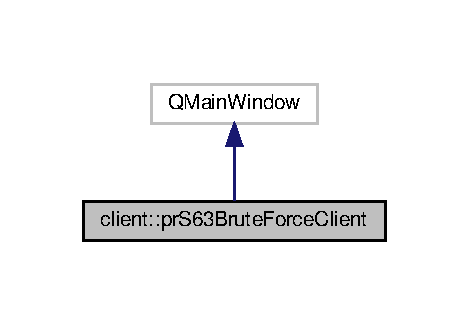
\includegraphics[width=225pt]{classclient_1_1pr_s63_brute_force_client__inherit__graph}
\end{center}
\end{figure}


Collaboration diagram for client\+:\+:pr\+S63\+Brute\+Force\+Client\+:\nopagebreak
\begin{figure}[H]
\begin{center}
\leavevmode
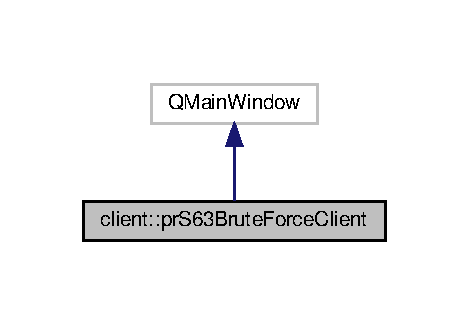
\includegraphics[width=225pt]{classclient_1_1pr_s63_brute_force_client__coll__graph}
\end{center}
\end{figure}
\subsection*{Public Member Functions}
\begin{DoxyCompactItemize}
\item 
\mbox{\Hypertarget{classclient_1_1pr_s63_brute_force_client_afa4597562e1bc7baa938d6fb29989d25}\label{classclient_1_1pr_s63_brute_force_client_afa4597562e1bc7baa938d6fb29989d25}} 
{\bfseries pr\+S63\+Brute\+Force\+Client} (Q\+Widget $\ast$parent=0)
\end{DoxyCompactItemize}


\subsection{Detailed Description}
Форма главного окна клиента для подбора пароля. 

Описание работы клиента находится в файле readme.\+md 

The documentation for this class was generated from the following files\+:\begin{DoxyCompactItemize}
\item 
/home/antonov/work\+Project/pr\+S63\+Brute\+Force/client/pr\+S63\+Brute\+Force\+Client/pr\+S63\+Brute\+Force\+Client.\+hpp\item 
/home/antonov/work\+Project/pr\+S63\+Brute\+Force/client/pr\+S63\+Brute\+Force\+Client/pr\+S63\+Brute\+Force\+Client.\+cpp\end{DoxyCompactItemize}

\hypertarget{classserver_1_1pr_s63_brute_force_server}{}\section{server\+:\+:pr\+S63\+Brute\+Force\+Server Class Reference}
\label{classserver_1_1pr_s63_brute_force_server}\index{server\+::pr\+S63\+Brute\+Force\+Server@{server\+::pr\+S63\+Brute\+Force\+Server}}


Inheritance diagram for server\+:\+:pr\+S63\+Brute\+Force\+Server\+:\nopagebreak
\begin{figure}[H]
\begin{center}
\leavevmode
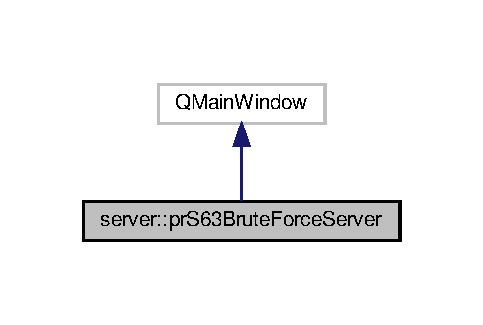
\includegraphics[width=232pt]{classserver_1_1pr_s63_brute_force_server__inherit__graph}
\end{center}
\end{figure}


Collaboration diagram for server\+:\+:pr\+S63\+Brute\+Force\+Server\+:\nopagebreak
\begin{figure}[H]
\begin{center}
\leavevmode
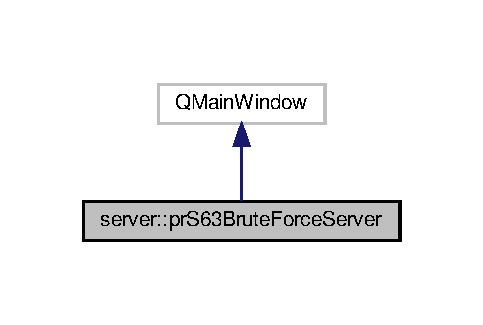
\includegraphics[width=232pt]{classserver_1_1pr_s63_brute_force_server__coll__graph}
\end{center}
\end{figure}
\subsection*{Public Member Functions}
\begin{DoxyCompactItemize}
\item 
\mbox{\Hypertarget{classserver_1_1pr_s63_brute_force_server_a50d074ec310fd67ed64de5bce5cff5ab}\label{classserver_1_1pr_s63_brute_force_server_a50d074ec310fd67ed64de5bce5cff5ab}} 
{\bfseries pr\+S63\+Brute\+Force\+Server} (Q\+Widget $\ast$parent=nullptr)
\end{DoxyCompactItemize}


The documentation for this class was generated from the following files\+:\begin{DoxyCompactItemize}
\item 
/home/antonov/work\+Project/pr\+S63\+Brute\+Force/server/pr\+S63\+Brute\+Force\+Server/pr\+S63\+Brute\+Force\+Server.\+hpp\item 
/home/antonov/work\+Project/pr\+S63\+Brute\+Force/server/pr\+S63\+Brute\+Force\+Server/pr\+S63\+Brute\+Force\+Server.\+cpp\end{DoxyCompactItemize}

\hypertarget{classblowfish_lib_1_1_t_blowfish}{}\section{blowfish\+Lib\+:\+:T\+Blowfish Class Reference}
\label{classblowfish_lib_1_1_t_blowfish}\index{blowfish\+Lib\+::\+T\+Blowfish@{blowfish\+Lib\+::\+T\+Blowfish}}


Класс выполняющий декодирование S63 и запись файла S57.  




{\ttfamily \#include $<$/home/antonov/work\+Project/pr\+S63\+Brute\+Force/lib/blowfish/\+T\+Blowfish.\+hpp$>$}

\subsection*{Public Member Functions}
\begin{DoxyCompactItemize}
\item 
\hyperlink{classblowfish_lib_1_1_t_blowfish_a349e59d7c45d5675376b89def7500c16}{T\+Blowfish} (td\+Ptr\+Buf, quint32)
\begin{DoxyCompactList}\small\item\em \hyperlink{classblowfish_lib_1_1_t_blowfish_a349e59d7c45d5675376b89def7500c16}{T\+Blowfish\+::\+T\+Blowfish} Конструктор класса \end{DoxyCompactList}\item 
\mbox{\Hypertarget{classblowfish_lib_1_1_t_blowfish_ad9ca35f3391415f31a265c440d63bf7f}\label{classblowfish_lib_1_1_t_blowfish_ad9ca35f3391415f31a265c440d63bf7f}} 
\hyperlink{classblowfish_lib_1_1_t_blowfish_ad9ca35f3391415f31a265c440d63bf7f}{T\+Blowfish} ()
\begin{DoxyCompactList}\small\item\em \hyperlink{classblowfish_lib_1_1_t_blowfish_a349e59d7c45d5675376b89def7500c16}{T\+Blowfish\+::\+T\+Blowfish} Конструктор класса \end{DoxyCompactList}\item 
\mbox{\Hypertarget{classblowfish_lib_1_1_t_blowfish_a2e410b2e410752f3ba96296fbcce9df2}\label{classblowfish_lib_1_1_t_blowfish_a2e410b2e410752f3ba96296fbcce9df2}} 
void \hyperlink{classblowfish_lib_1_1_t_blowfish_a2e410b2e410752f3ba96296fbcce9df2}{clear} ()
\begin{DoxyCompactList}\small\item\em \hyperlink{classblowfish_lib_1_1_t_blowfish_a2e410b2e410752f3ba96296fbcce9df2}{T\+Blowfish\+::clear} Очистка всех данных \end{DoxyCompactList}\item 
void \hyperlink{classblowfish_lib_1_1_t_blowfish_aac58cd909cef267ba409859c279dc521}{set\+Data} (td\+Ptr\+Buf, quint32)
\begin{DoxyCompactList}\small\item\em \hyperlink{classblowfish_lib_1_1_t_blowfish_aac58cd909cef267ba409859c279dc521}{T\+Blowfish\+::set\+Data} Установка буфера с данными. \end{DoxyCompactList}\item 
bool \hyperlink{classblowfish_lib_1_1_t_blowfish_a5bb77f2618aa5dd97b86d842e546fdae}{decrypt\+Part} (Q\+String)
\begin{DoxyCompactList}\small\item\em \hyperlink{classblowfish_lib_1_1_t_blowfish_a5bb77f2618aa5dd97b86d842e546fdae}{T\+Blowfish\+::decrypt\+Part} Расшифровка первых 8-\/ми байт массива. \end{DoxyCompactList}\item 
bool \hyperlink{classblowfish_lib_1_1_t_blowfish_aa6cf535926e4a3daae058725a6192619}{decrypt\+Full} (Q\+String)
\begin{DoxyCompactList}\small\item\em \hyperlink{classblowfish_lib_1_1_t_blowfish_aa6cf535926e4a3daae058725a6192619}{T\+Blowfish\+::decrypt\+Full} Полная расшифровка буфера \end{DoxyCompactList}\item 
bool \hyperlink{classblowfish_lib_1_1_t_blowfish_a17896279118b13a237ab31c1cb82da26}{unzip} ()
\begin{DoxyCompactList}\small\item\em \hyperlink{classblowfish_lib_1_1_t_blowfish_a17896279118b13a237ab31c1cb82da26}{T\+Blowfish\+::unzip} Разархивация декодированного буфера \end{DoxyCompactList}\item 
\mbox{\Hypertarget{classblowfish_lib_1_1_t_blowfish_a0e634baff0aba9677a41c58c01a6b25a}\label{classblowfish_lib_1_1_t_blowfish_a0e634baff0aba9677a41c58c01a6b25a}} 
void {\bfseries write\+File} (Q\+String)
\item 
td\+Ptr\+Buf \hyperlink{classblowfish_lib_1_1_t_blowfish_ab1f9fc3cc9b075c3b9b558b5719c159e}{get\+Decrypt\+Buf} ()
\begin{DoxyCompactList}\small\item\em get\+Decrypt\+Buf Возвращает дешифрованный буфер. Размер буфера равен исходному. \end{DoxyCompactList}\item 
bool \hyperlink{classblowfish_lib_1_1_t_blowfish_a53eba59c588fafe24260a0cf05b7866b}{check\+Decrypt} ()
\begin{DoxyCompactList}\small\item\em \hyperlink{classblowfish_lib_1_1_t_blowfish_a53eba59c588fafe24260a0cf05b7866b}{T\+Blowfish\+::check\+Decrypt} Проверка сигнатуры zip-\/файл 0x04034\+B50 в первых 4х байтах \end{DoxyCompactList}\end{DoxyCompactItemize}


\subsection{Detailed Description}
Класс выполняющий декодирование S63 и запись файла S57. 

\subsection{Constructor \& Destructor Documentation}
\mbox{\Hypertarget{classblowfish_lib_1_1_t_blowfish_a349e59d7c45d5675376b89def7500c16}\label{classblowfish_lib_1_1_t_blowfish_a349e59d7c45d5675376b89def7500c16}} 
\index{blowfish\+Lib\+::\+T\+Blowfish@{blowfish\+Lib\+::\+T\+Blowfish}!T\+Blowfish@{T\+Blowfish}}
\index{T\+Blowfish@{T\+Blowfish}!blowfish\+Lib\+::\+T\+Blowfish@{blowfish\+Lib\+::\+T\+Blowfish}}
\subsubsection{\texorpdfstring{T\+Blowfish()}{TBlowfish()}}
{\footnotesize\ttfamily T\+Blowfish\+::\+T\+Blowfish (\begin{DoxyParamCaption}\item[{td\+Ptr\+Buf}]{in\+Ptr\+Buf,  }\item[{quint32}]{in\+Buf\+Size }\end{DoxyParamCaption})}



\hyperlink{classblowfish_lib_1_1_t_blowfish_a349e59d7c45d5675376b89def7500c16}{T\+Blowfish\+::\+T\+Blowfish} Конструктор класса 


\begin{DoxyParams}{Parameters}
{\em in\+Ptr\+Buf} & Указатель на массив данных которые нужно расшифровать и разархивировать \\
\hline
{\em in\+Buf\+Size} & Размер данного буфера \\
\hline
\end{DoxyParams}


\subsection{Member Function Documentation}
\mbox{\Hypertarget{classblowfish_lib_1_1_t_blowfish_a53eba59c588fafe24260a0cf05b7866b}\label{classblowfish_lib_1_1_t_blowfish_a53eba59c588fafe24260a0cf05b7866b}} 
\index{blowfish\+Lib\+::\+T\+Blowfish@{blowfish\+Lib\+::\+T\+Blowfish}!check\+Decrypt@{check\+Decrypt}}
\index{check\+Decrypt@{check\+Decrypt}!blowfish\+Lib\+::\+T\+Blowfish@{blowfish\+Lib\+::\+T\+Blowfish}}
\subsubsection{\texorpdfstring{check\+Decrypt()}{checkDecrypt()}}
{\footnotesize\ttfamily bool T\+Blowfish\+::check\+Decrypt (\begin{DoxyParamCaption}{ }\end{DoxyParamCaption})}



\hyperlink{classblowfish_lib_1_1_t_blowfish_a53eba59c588fafe24260a0cf05b7866b}{T\+Blowfish\+::check\+Decrypt} Проверка сигнатуры zip-\/файл 0x04034\+B50 в первых 4х байтах 

\begin{DoxyReturn}{Returns}
Если сигнатура 
\end{DoxyReturn}
\mbox{\Hypertarget{classblowfish_lib_1_1_t_blowfish_aa6cf535926e4a3daae058725a6192619}\label{classblowfish_lib_1_1_t_blowfish_aa6cf535926e4a3daae058725a6192619}} 
\index{blowfish\+Lib\+::\+T\+Blowfish@{blowfish\+Lib\+::\+T\+Blowfish}!decrypt\+Full@{decrypt\+Full}}
\index{decrypt\+Full@{decrypt\+Full}!blowfish\+Lib\+::\+T\+Blowfish@{blowfish\+Lib\+::\+T\+Blowfish}}
\subsubsection{\texorpdfstring{decrypt\+Full()}{decryptFull()}}
{\footnotesize\ttfamily bool T\+Blowfish\+::decrypt\+Full (\begin{DoxyParamCaption}\item[{Q\+String}]{in\+Key }\end{DoxyParamCaption})}



\hyperlink{classblowfish_lib_1_1_t_blowfish_aa6cf535926e4a3daae058725a6192619}{T\+Blowfish\+::decrypt\+Full} Полная расшифровка буфера 


\begin{DoxyParams}{Parameters}
{\em in\+Key} & Ключ для расшифровки \\
\hline
\end{DoxyParams}
\begin{DoxyReturn}{Returns}
В случае получения сигнатуры zip файла, возвращает true
\end{DoxyReturn}
Проверка декодирования выполняется только по первым 4 байтам на соответствие сигнатуре zip файла. Для полной проверки правильности дешифрации нужно выполнить разархивацию файла. \mbox{\Hypertarget{classblowfish_lib_1_1_t_blowfish_a5bb77f2618aa5dd97b86d842e546fdae}\label{classblowfish_lib_1_1_t_blowfish_a5bb77f2618aa5dd97b86d842e546fdae}} 
\index{blowfish\+Lib\+::\+T\+Blowfish@{blowfish\+Lib\+::\+T\+Blowfish}!decrypt\+Part@{decrypt\+Part}}
\index{decrypt\+Part@{decrypt\+Part}!blowfish\+Lib\+::\+T\+Blowfish@{blowfish\+Lib\+::\+T\+Blowfish}}
\subsubsection{\texorpdfstring{decrypt\+Part()}{decryptPart()}}
{\footnotesize\ttfamily bool T\+Blowfish\+::decrypt\+Part (\begin{DoxyParamCaption}\item[{Q\+String}]{in\+Key }\end{DoxyParamCaption})}



\hyperlink{classblowfish_lib_1_1_t_blowfish_a5bb77f2618aa5dd97b86d842e546fdae}{T\+Blowfish\+::decrypt\+Part} Расшифровка первых 8-\/ми байт массива. 


\begin{DoxyParams}{Parameters}
{\em in\+Key} & Ключ для расшифровки \\
\hline
\end{DoxyParams}
\begin{DoxyReturn}{Returns}
В случае получения сигнатуры zip файла, возвращает true 
\end{DoxyReturn}
\mbox{\Hypertarget{classblowfish_lib_1_1_t_blowfish_ab1f9fc3cc9b075c3b9b558b5719c159e}\label{classblowfish_lib_1_1_t_blowfish_ab1f9fc3cc9b075c3b9b558b5719c159e}} 
\index{blowfish\+Lib\+::\+T\+Blowfish@{blowfish\+Lib\+::\+T\+Blowfish}!get\+Decrypt\+Buf@{get\+Decrypt\+Buf}}
\index{get\+Decrypt\+Buf@{get\+Decrypt\+Buf}!blowfish\+Lib\+::\+T\+Blowfish@{blowfish\+Lib\+::\+T\+Blowfish}}
\subsubsection{\texorpdfstring{get\+Decrypt\+Buf()}{getDecryptBuf()}}
{\footnotesize\ttfamily td\+Ptr\+Buf T\+Blowfish\+::get\+Decrypt\+Buf (\begin{DoxyParamCaption}{ }\end{DoxyParamCaption})}



get\+Decrypt\+Buf Возвращает дешифрованный буфер. Размер буфера равен исходному. 

\begin{DoxyReturn}{Returns}
Указатель на буфер с преобразованными данными 
\end{DoxyReturn}
\mbox{\Hypertarget{classblowfish_lib_1_1_t_blowfish_aac58cd909cef267ba409859c279dc521}\label{classblowfish_lib_1_1_t_blowfish_aac58cd909cef267ba409859c279dc521}} 
\index{blowfish\+Lib\+::\+T\+Blowfish@{blowfish\+Lib\+::\+T\+Blowfish}!set\+Data@{set\+Data}}
\index{set\+Data@{set\+Data}!blowfish\+Lib\+::\+T\+Blowfish@{blowfish\+Lib\+::\+T\+Blowfish}}
\subsubsection{\texorpdfstring{set\+Data()}{setData()}}
{\footnotesize\ttfamily void T\+Blowfish\+::set\+Data (\begin{DoxyParamCaption}\item[{td\+Ptr\+Buf}]{in\+Ptr\+Buf,  }\item[{quint32}]{in\+Buf\+Size }\end{DoxyParamCaption})}



\hyperlink{classblowfish_lib_1_1_t_blowfish_aac58cd909cef267ba409859c279dc521}{T\+Blowfish\+::set\+Data} Установка буфера с данными. 


\begin{DoxyParams}{Parameters}
{\em in\+Ptr\+Buf} & Указатель на массив данных которые нужно расшифровать и разархивировать \\
\hline
{\em in\+Buf\+Size} & Размер данного буфера \\
\hline
\end{DoxyParams}
\mbox{\Hypertarget{classblowfish_lib_1_1_t_blowfish_a17896279118b13a237ab31c1cb82da26}\label{classblowfish_lib_1_1_t_blowfish_a17896279118b13a237ab31c1cb82da26}} 
\index{blowfish\+Lib\+::\+T\+Blowfish@{blowfish\+Lib\+::\+T\+Blowfish}!unzip@{unzip}}
\index{unzip@{unzip}!blowfish\+Lib\+::\+T\+Blowfish@{blowfish\+Lib\+::\+T\+Blowfish}}
\subsubsection{\texorpdfstring{unzip()}{unzip()}}
{\footnotesize\ttfamily bool T\+Blowfish\+::unzip (\begin{DoxyParamCaption}{ }\end{DoxyParamCaption})}



\hyperlink{classblowfish_lib_1_1_t_blowfish_a17896279118b13a237ab31c1cb82da26}{T\+Blowfish\+::unzip} Разархивация декодированного буфера 

\begin{DoxyReturn}{Returns}
Вслучаем успешной разархивации возвращается true
\end{DoxyReturn}
Для разврхивации используется zlib. В дальнейшем, если возможно, то нужно переделать на использование Botan\+::\+Zlib\+\_\+\+Decompression 

The documentation for this class was generated from the following files\+:\begin{DoxyCompactItemize}
\item 
/home/antonov/work\+Project/pr\+S63\+Brute\+Force/lib/blowfish/T\+Blowfish.\+hpp\item 
/home/antonov/work\+Project/pr\+S63\+Brute\+Force/lib/blowfish/T\+Blowfish.\+cpp\end{DoxyCompactItemize}

\hypertarget{classblowfish_lib_1_1blowfish_exeption_1_1_t_blowfish_exeption}{}\section{blowfish\+Lib\+:\+:blowfish\+Exeption\+:\+:T\+Blowfish\+Exeption Class Reference}
\label{classblowfish_lib_1_1blowfish_exeption_1_1_t_blowfish_exeption}\index{blowfish\+Lib\+::blowfish\+Exeption\+::\+T\+Blowfish\+Exeption@{blowfish\+Lib\+::blowfish\+Exeption\+::\+T\+Blowfish\+Exeption}}


Класс обработки ошибок при декодировании  




{\ttfamily \#include $<$/home/antonov/work\+Project/pr\+S63\+Brute\+Force/lib/blowfish/\+T\+Blowfish.\+hpp$>$}



Inheritance diagram for blowfish\+Lib\+:\+:blowfish\+Exeption\+:\+:T\+Blowfish\+Exeption\+:
\nopagebreak
\begin{figure}[H]
\begin{center}
\leavevmode
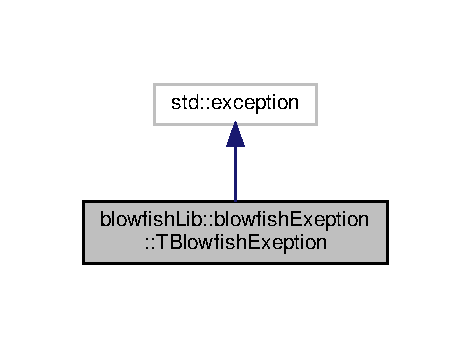
\includegraphics[width=226pt]{classblowfish_lib_1_1blowfish_exeption_1_1_t_blowfish_exeption__inherit__graph}
\end{center}
\end{figure}


Collaboration diagram for blowfish\+Lib\+:\+:blowfish\+Exeption\+:\+:T\+Blowfish\+Exeption\+:
\nopagebreak
\begin{figure}[H]
\begin{center}
\leavevmode
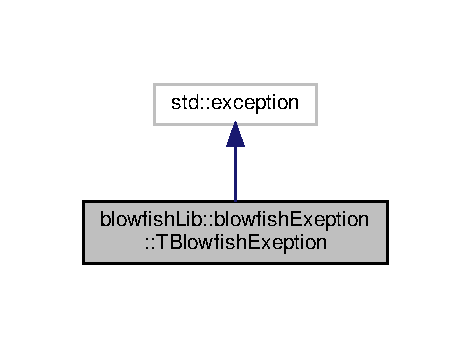
\includegraphics[width=226pt]{classblowfish_lib_1_1blowfish_exeption_1_1_t_blowfish_exeption__coll__graph}
\end{center}
\end{figure}
\subsection*{Public Member Functions}
\begin{DoxyCompactItemize}
\item 
\mbox{\Hypertarget{classblowfish_lib_1_1blowfish_exeption_1_1_t_blowfish_exeption_abf34d81a97e5611cbde29e4f9d392c19}\label{classblowfish_lib_1_1blowfish_exeption_1_1_t_blowfish_exeption_abf34d81a97e5611cbde29e4f9d392c19}} 
{\bfseries T\+Blowfish\+Exeption} (std\+::error\+\_\+code in\+Error\+Code, std\+::string in\+Text\+Error)
\item 
\mbox{\Hypertarget{classblowfish_lib_1_1blowfish_exeption_1_1_t_blowfish_exeption_a9f760be4de799f9010c1552361df8dd3}\label{classblowfish_lib_1_1blowfish_exeption_1_1_t_blowfish_exeption_a9f760be4de799f9010c1552361df8dd3}} 
const char $\ast$ {\bfseries what} () const  throw ()
\item 
\mbox{\Hypertarget{classblowfish_lib_1_1blowfish_exeption_1_1_t_blowfish_exeption_a95b80b0c4eba5a8951022e70849cd116}\label{classblowfish_lib_1_1blowfish_exeption_1_1_t_blowfish_exeption_a95b80b0c4eba5a8951022e70849cd116}} 
const std\+::error\+\_\+code \& {\bfseries code} () const noexcept
\end{DoxyCompactItemize}


\subsection{Detailed Description}
Класс обработки ошибок при декодировании 

The documentation for this class was generated from the following file\+:\begin{DoxyCompactItemize}
\item 
/home/antonov/work\+Project/pr\+S63\+Brute\+Force/lib/blowfish/T\+Blowfish.\+hpp\end{DoxyCompactItemize}

\hypertarget{structblowfish_lib_1_1blowfish_exeption_1_1_t_blowfish_exeption_category}{}\section{blowfish\+Lib\+:\+:blowfish\+Exeption\+:\+:T\+Blowfish\+Exeption\+Category Struct Reference}
\label{structblowfish_lib_1_1blowfish_exeption_1_1_t_blowfish_exeption_category}\index{blowfish\+Lib\+::blowfish\+Exeption\+::\+T\+Blowfish\+Exeption\+Category@{blowfish\+Lib\+::blowfish\+Exeption\+::\+T\+Blowfish\+Exeption\+Category}}


Структура для формирования std\+::error\+\_\+code для класса декодирования  




{\ttfamily \#include $<$/home/antonov/work\+Project/pr\+S63\+Brute\+Force/lib/blowfish/\+T\+Blowfish.\+hpp$>$}



Inheritance diagram for blowfish\+Lib\+:\+:blowfish\+Exeption\+:\+:T\+Blowfish\+Exeption\+Category\+:
\nopagebreak
\begin{figure}[H]
\begin{center}
\leavevmode
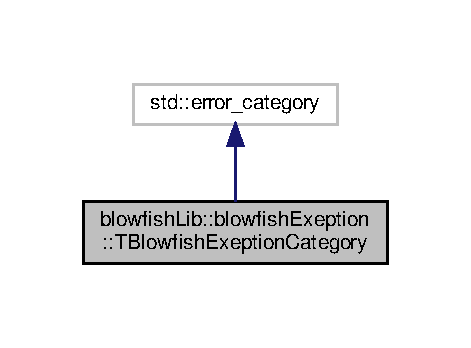
\includegraphics[width=226pt]{structblowfish_lib_1_1blowfish_exeption_1_1_t_blowfish_exeption_category__inherit__graph}
\end{center}
\end{figure}


Collaboration diagram for blowfish\+Lib\+:\+:blowfish\+Exeption\+:\+:T\+Blowfish\+Exeption\+Category\+:
\nopagebreak
\begin{figure}[H]
\begin{center}
\leavevmode
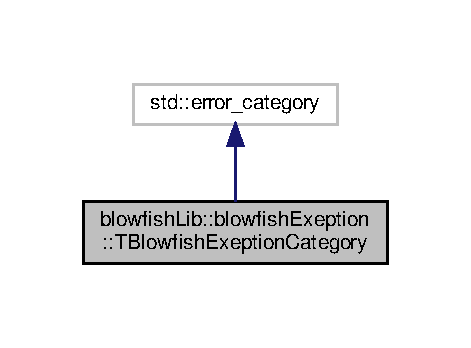
\includegraphics[width=226pt]{structblowfish_lib_1_1blowfish_exeption_1_1_t_blowfish_exeption_category__coll__graph}
\end{center}
\end{figure}
\subsection*{Public Member Functions}
\begin{DoxyCompactItemize}
\item 
\mbox{\Hypertarget{structblowfish_lib_1_1blowfish_exeption_1_1_t_blowfish_exeption_category_a92923b786609d0b69a7ce3ab709d0e2c}\label{structblowfish_lib_1_1blowfish_exeption_1_1_t_blowfish_exeption_category_a92923b786609d0b69a7ce3ab709d0e2c}} 
const char $\ast$ {\bfseries name} () const noexcept
\item 
\mbox{\Hypertarget{structblowfish_lib_1_1blowfish_exeption_1_1_t_blowfish_exeption_category_ac1f3b94e050e69b92bd51af85b9f8ea6}\label{structblowfish_lib_1_1blowfish_exeption_1_1_t_blowfish_exeption_category_ac1f3b94e050e69b92bd51af85b9f8ea6}} 
std\+::string {\bfseries message} (int in\+Ex=0) const
\end{DoxyCompactItemize}


\subsection{Detailed Description}
Структура для формирования std\+::error\+\_\+code для класса декодирования 

The documentation for this struct was generated from the following file\+:\begin{DoxyCompactItemize}
\item 
/home/antonov/work\+Project/pr\+S63\+Brute\+Force/lib/blowfish/T\+Blowfish.\+hpp\end{DoxyCompactItemize}

\hypertarget{classserver_1_1_t_brute_force_manager}{}\section{server\+:\+:T\+Brute\+Force\+Manager Class Reference}
\label{classserver_1_1_t_brute_force_manager}\index{server\+::\+T\+Brute\+Force\+Manager@{server\+::\+T\+Brute\+Force\+Manager}}


Класс выполняющий распределение блоков между клиентами  




{\ttfamily \#include $<$T\+Brute\+Force\+Manager.\+hpp$>$}



Inheritance diagram for server\+:\+:T\+Brute\+Force\+Manager\+:\nopagebreak
\begin{figure}[H]
\begin{center}
\leavevmode
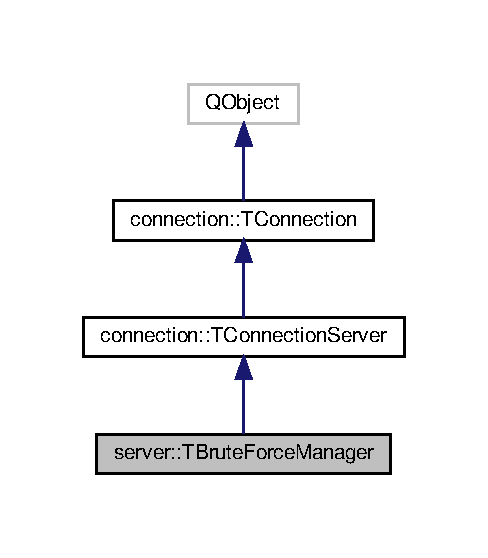
\includegraphics[width=234pt]{classserver_1_1_t_brute_force_manager__inherit__graph}
\end{center}
\end{figure}


Collaboration diagram for server\+:\+:T\+Brute\+Force\+Manager\+:\nopagebreak
\begin{figure}[H]
\begin{center}
\leavevmode
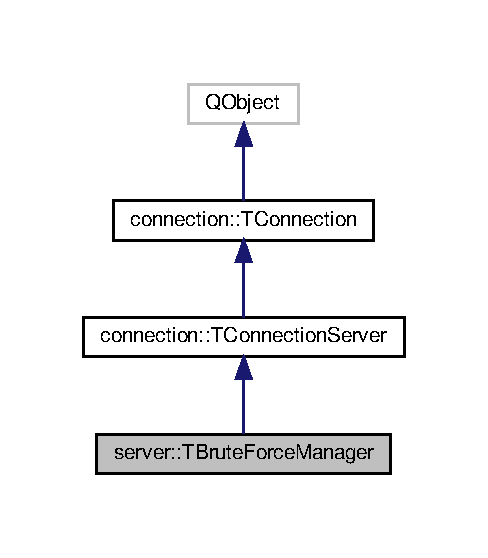
\includegraphics[width=234pt]{classserver_1_1_t_brute_force_manager__coll__graph}
\end{center}
\end{figure}
\subsection*{Public Member Functions}
\begin{DoxyCompactItemize}
\item 
\mbox{\Hypertarget{classserver_1_1_t_brute_force_manager_ac7c9f1590534d38fe05c422e7fada979}\label{classserver_1_1_t_brute_force_manager_ac7c9f1590534d38fe05c422e7fada979}} 
\hyperlink{classserver_1_1_t_brute_force_manager_ac7c9f1590534d38fe05c422e7fada979}{T\+Brute\+Force\+Manager} ()
\begin{DoxyCompactList}\small\item\em \hyperlink{classserver_1_1_t_brute_force_manager_ac7c9f1590534d38fe05c422e7fada979}{T\+Brute\+Force\+Manager\+::\+T\+Brute\+Force\+Manager} Конструктор класса \end{DoxyCompactList}\end{DoxyCompactItemize}
\subsection*{Additional Inherited Members}


\subsection{Detailed Description}
Класс выполняющий распределение блоков между клиентами 

The documentation for this class was generated from the following files\+:\begin{DoxyCompactItemize}
\item 
server/pr\+S63\+Brute\+Force\+Server/T\+Brute\+Force\+Manager.\+hpp\item 
server/pr\+S63\+Brute\+Force\+Server/T\+Brute\+Force\+Manager.\+cpp\end{DoxyCompactItemize}

\hypertarget{classclient_1_1_t_client_model}{}\section{client\+:\+:T\+Client\+Model Class Reference}
\label{classclient_1_1_t_client_model}\index{client\+::\+T\+Client\+Model@{client\+::\+T\+Client\+Model}}


The \hyperlink{classclient_1_1_t_client_model}{T\+Client\+Model} class Модель для отображения лога работы клиентов  




{\ttfamily \#include $<$T\+Client\+Model.\+hpp$>$}



Inheritance diagram for client\+:\+:T\+Client\+Model\+:\nopagebreak
\begin{figure}[H]
\begin{center}
\leavevmode
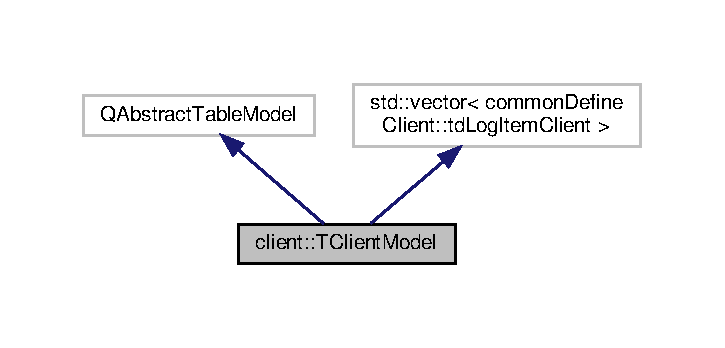
\includegraphics[width=348pt]{classclient_1_1_t_client_model__inherit__graph}
\end{center}
\end{figure}


Collaboration diagram for client\+:\+:T\+Client\+Model\+:\nopagebreak
\begin{figure}[H]
\begin{center}
\leavevmode
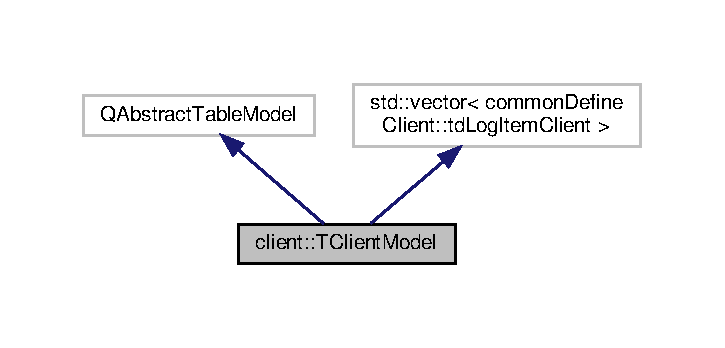
\includegraphics[width=348pt]{classclient_1_1_t_client_model__coll__graph}
\end{center}
\end{figure}
\subsection*{Public Member Functions}
\begin{DoxyCompactItemize}
\item 
\mbox{\Hypertarget{classclient_1_1_t_client_model_a56d1ca59a519931a703e024698c83a42}\label{classclient_1_1_t_client_model_a56d1ca59a519931a703e024698c83a42}} 
\hyperlink{classclient_1_1_t_client_model_a56d1ca59a519931a703e024698c83a42}{T\+Client\+Model} (quint16 in\+Thread\+Count, Q\+Object $\ast$parent=nullptr)
\begin{DoxyCompactList}\small\item\em \hyperlink{classclient_1_1_t_client_model_a56d1ca59a519931a703e024698c83a42}{T\+Client\+Model\+::\+T\+Client\+Model} Конструктор модели \end{DoxyCompactList}\item 
\mbox{\Hypertarget{classclient_1_1_t_client_model_a282427450592390fce094bdc9645b00f}\label{classclient_1_1_t_client_model_a282427450592390fce094bdc9645b00f}} 
int {\bfseries row\+Count} (const Q\+Model\+Index \&parent) const
\item 
\mbox{\Hypertarget{classclient_1_1_t_client_model_ada4b178e21da50180ec36f2faf8e89d2}\label{classclient_1_1_t_client_model_ada4b178e21da50180ec36f2faf8e89d2}} 
int {\bfseries column\+Count} (const Q\+Model\+Index \&parent=Q\+Model\+Index()) const
\item 
\mbox{\Hypertarget{classclient_1_1_t_client_model_ac8203af327c334a6b28bddd2c2f4626c}\label{classclient_1_1_t_client_model_ac8203af327c334a6b28bddd2c2f4626c}} 
Q\+Variant {\bfseries data} (const Q\+Model\+Index \&index, int role) const
\item 
\mbox{\Hypertarget{classclient_1_1_t_client_model_a3e5645fece3531d74e2961968a3ea597}\label{classclient_1_1_t_client_model_a3e5645fece3531d74e2961968a3ea597}} 
Q\+Variant {\bfseries header\+Data} (int section, Qt\+::\+Orientation orientation, int role=Qt\+::\+Display\+Role) const
\item 
void \hyperlink{classclient_1_1_t_client_model_aed00383c6177d60cb6f4b34b23fce485}{push\+\_\+back} (common\+Define\+Client\+::td\+Log\+Item\+Client)
\begin{DoxyCompactList}\small\item\em \hyperlink{classclient_1_1_t_client_model_aed00383c6177d60cb6f4b34b23fce485}{client\+::\+T\+Client\+Model\+::push\+\_\+back} Добавляем в модель запись о сгенерированном числе. \end{DoxyCompactList}\item 
\mbox{\Hypertarget{classclient_1_1_t_client_model_aea0cb37f9e91c028f699e4da3663fcea}\label{classclient_1_1_t_client_model_aea0cb37f9e91c028f699e4da3663fcea}} 
void \hyperlink{classclient_1_1_t_client_model_aea0cb37f9e91c028f699e4da3663fcea}{refresh\+View} ()
\begin{DoxyCompactList}\small\item\em \hyperlink{classclient_1_1_t_client_model_aea0cb37f9e91c028f699e4da3663fcea}{client\+::\+T\+Client\+Model\+::refresh\+View} Обновление отображения данных \end{DoxyCompactList}\end{DoxyCompactItemize}


\subsection{Detailed Description}
The \hyperlink{classclient_1_1_t_client_model}{T\+Client\+Model} class Модель для отображения лога работы клиентов 

\subsection{Member Function Documentation}
\mbox{\Hypertarget{classclient_1_1_t_client_model_aed00383c6177d60cb6f4b34b23fce485}\label{classclient_1_1_t_client_model_aed00383c6177d60cb6f4b34b23fce485}} 
\index{client\+::\+T\+Client\+Model@{client\+::\+T\+Client\+Model}!push\+\_\+back@{push\+\_\+back}}
\index{push\+\_\+back@{push\+\_\+back}!client\+::\+T\+Client\+Model@{client\+::\+T\+Client\+Model}}
\subsubsection{\texorpdfstring{push\+\_\+back()}{push\_back()}}
{\footnotesize\ttfamily void client\+::\+T\+Client\+Model\+::push\+\_\+back (\begin{DoxyParamCaption}\item[{common\+Define\+Client\+::td\+Log\+Item\+Client}]{in\+Item }\end{DoxyParamCaption})}



\hyperlink{classclient_1_1_t_client_model_aed00383c6177d60cb6f4b34b23fce485}{client\+::\+T\+Client\+Model\+::push\+\_\+back} Добавляем в модель запись о сгенерированном числе. 


\begin{DoxyParams}{Parameters}
{\em in\+Item} & Унказатель на добавляемая запись\\
\hline
\end{DoxyParams}
Обновлять данные в этот момент нельзя, т.\+к. при очистке контейнера софт может обновлять отображение данных и т.\+о. будет падать. 

The documentation for this class was generated from the following files\+:\begin{DoxyCompactItemize}
\item 
client/pr\+S63\+Brute\+Force\+Client/T\+Client\+Model.\+hpp\item 
client/pr\+S63\+Brute\+Force\+Client/T\+Client\+Model.\+cpp\end{DoxyCompactItemize}

\hypertarget{classconnection_1_1_t_connection}{}\section{connection\+:\+:T\+Connection Class Reference}
\label{classconnection_1_1_t_connection}\index{connection\+::\+T\+Connection@{connection\+::\+T\+Connection}}


The \hyperlink{classconnection_1_1_t_connection}{T\+Connection} class Базовый класс для обслуживания работы распределенной системы  




{\ttfamily \#include $<$/home/antonov/work\+Project/pr\+S63\+Brute\+Force/common/\+T\+Connection.\+hpp$>$}



Inheritance diagram for connection\+:\+:T\+Connection\+:\nopagebreak
\begin{figure}[H]
\begin{center}
\leavevmode
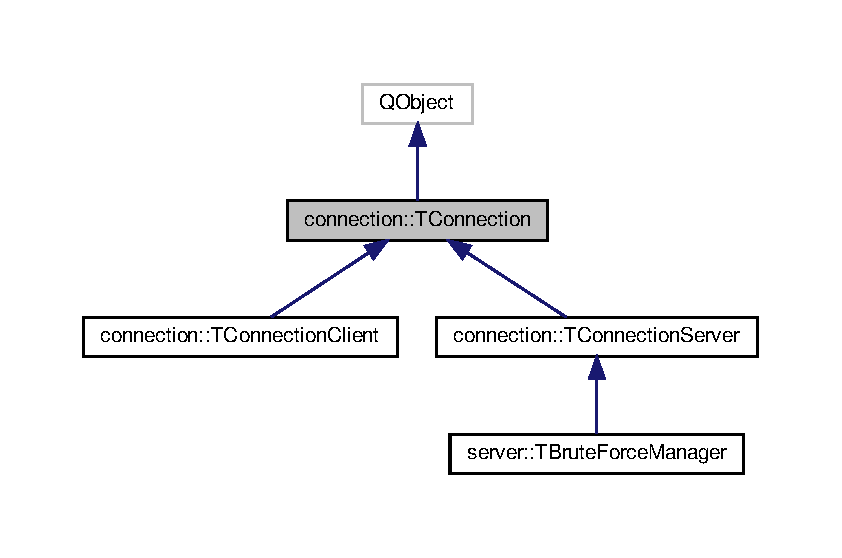
\includegraphics[width=350pt]{classconnection_1_1_t_connection__inherit__graph}
\end{center}
\end{figure}


Collaboration diagram for connection\+:\+:T\+Connection\+:\nopagebreak
\begin{figure}[H]
\begin{center}
\leavevmode
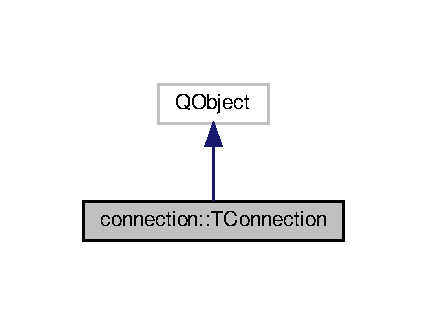
\includegraphics[width=205pt]{classconnection_1_1_t_connection__coll__graph}
\end{center}
\end{figure}
\subsection*{Public Types}
\begin{DoxyCompactItemize}
\item 
enum \hyperlink{classconnection_1_1_t_connection_a3550181cb2fa72eccfa55d23f45cea34}{exchange\+Protocol} \{ \newline
\hyperlink{classconnection_1_1_t_connection_a3550181cb2fa72eccfa55d23f45cea34a70f4e9439076a2b1cdc0f89b0f3e81cb}{cmd\+Unknown}, 
\hyperlink{classconnection_1_1_t_connection_a3550181cb2fa72eccfa55d23f45cea34a17295bd27841a9cb3ad942201087e366}{cmd\+Connection\+Request}, 
\hyperlink{classconnection_1_1_t_connection_a3550181cb2fa72eccfa55d23f45cea34ab0cb460aa502bc429f7b5827d53bc80c}{cmd\+Connection\+Confirm}, 
\hyperlink{classconnection_1_1_t_connection_a3550181cb2fa72eccfa55d23f45cea34a03a1c4d18739819cbf74e5540c5da54d}{cmd\+Connection\+Close}, 
\newline
\hyperlink{classconnection_1_1_t_connection_a3550181cb2fa72eccfa55d23f45cea34a5f20bb0c4e68d19fedbb8f9c8c91f255}{cmd\+Transfer\+Data}, 
\hyperlink{classconnection_1_1_t_connection_a3550181cb2fa72eccfa55d23f45cea34a1b1480ee3f1a3727645610c6451c2d82}{cmd\+Accept\+Data}, 
\hyperlink{classconnection_1_1_t_connection_a3550181cb2fa72eccfa55d23f45cea34afa78af46af0ba99a38de59dddf750b8f}{cmd\+Refuse\+Data}, 
\hyperlink{classconnection_1_1_t_connection_a3550181cb2fa72eccfa55d23f45cea34acef0bc6c3064f9f5f9ff2c3f959c66a6}{cmd\+Transfer\+Request}, 
\newline
\hyperlink{classconnection_1_1_t_connection_a3550181cb2fa72eccfa55d23f45cea34ad56de56b3d7d7b5fa429869bdadc001a}{cmd\+State\+Request}, 
\hyperlink{classconnection_1_1_t_connection_a3550181cb2fa72eccfa55d23f45cea34a12b5301bb4cdfde5b03b189d639d3d88}{cmd\+State\+Confirm}, 
\hyperlink{classconnection_1_1_t_connection_a3550181cb2fa72eccfa55d23f45cea34a3f22bedf0adda5299a699d9dfe17b811}{cmd\+Count}
 \}\begin{DoxyCompactList}\small\item\em Протокол обмена между сервером и клиентами. \end{DoxyCompactList}
\item 
enum \hyperlink{classconnection_1_1_t_connection_aee7dfb7510592bd2697ab6f906b9612c}{state} \{ \newline
\hyperlink{classconnection_1_1_t_connection_aee7dfb7510592bd2697ab6f906b9612ca8ab66af10a4d089e45c493a28df001e4}{st\+Unknown}, 
\hyperlink{classconnection_1_1_t_connection_aee7dfb7510592bd2697ab6f906b9612ca718b9080d3864c424cc4e162554b7cea}{st\+Connected}, 
\hyperlink{classconnection_1_1_t_connection_aee7dfb7510592bd2697ab6f906b9612ca01c9bac9850308a008d1acba4c1a68b7}{st\+Disconnected}, 
\hyperlink{classconnection_1_1_t_connection_aee7dfb7510592bd2697ab6f906b9612caad14f181573f29386d8f394621abd498}{st\+Wait}, 
\newline
\hyperlink{classconnection_1_1_t_connection_aee7dfb7510592bd2697ab6f906b9612ca22858c36fed3fc0fd61036ac4ae07c16}{st\+Ready\+To\+Start}, 
\hyperlink{classconnection_1_1_t_connection_aee7dfb7510592bd2697ab6f906b9612cae8cadea9b3262d6021dc2dd5a8983b07}{st\+Not\+Ready\+To\+Start}, 
\hyperlink{classconnection_1_1_t_connection_aee7dfb7510592bd2697ab6f906b9612ca242131a52a37a2916e7292733c05bfda}{st\+Start}, 
\hyperlink{classconnection_1_1_t_connection_aee7dfb7510592bd2697ab6f906b9612caaef0b02f1701010c8b408087afbb1172}{st\+Stop}, 
\newline
\hyperlink{classconnection_1_1_t_connection_aee7dfb7510592bd2697ab6f906b9612ca67a6ae9e7f0931220dc51adc849cc41e}{st\+Error}, 
\hyperlink{classconnection_1_1_t_connection_aee7dfb7510592bd2697ab6f906b9612ca1429dfb087b4132ff51a6d083c452624}{st\+Server\+Search}, 
\hyperlink{classconnection_1_1_t_connection_aee7dfb7510592bd2697ab6f906b9612ca194b89ec7cadeb35331341be96c05f76}{st\+Pause}, 
\hyperlink{classconnection_1_1_t_connection_aee7dfb7510592bd2697ab6f906b9612ca4e5cb1da08e0cca3013f7fdbdf430273}{st\+App\+Close}
 \}\begin{DoxyCompactList}\small\item\em Возможные состояния \end{DoxyCompactList}
\end{DoxyCompactItemize}
\subsection*{Public Member Functions}
\begin{DoxyCompactItemize}
\item 
\mbox{\Hypertarget{classconnection_1_1_t_connection_a3457e15061be61110b825fd1760e3834}\label{classconnection_1_1_t_connection_a3457e15061be61110b825fd1760e3834}} 
\hyperlink{classconnection_1_1_t_connection_a3457e15061be61110b825fd1760e3834}{T\+Connection} ()
\begin{DoxyCompactList}\small\item\em \hyperlink{classconnection_1_1_t_connection_a3457e15061be61110b825fd1760e3834}{T\+Connection\+::\+T\+Connection} Конструктор класса \end{DoxyCompactList}\item 
\hyperlink{classconnection_1_1_t_connection_aee7dfb7510592bd2697ab6f906b9612c}{state} \hyperlink{classconnection_1_1_t_connection_a23088724b46efeed0ae8d0d6b1e738b1}{get\+State} ()
\begin{DoxyCompactList}\small\item\em \hyperlink{classconnection_1_1_t_connection_a23088724b46efeed0ae8d0d6b1e738b1}{T\+Connection\+::get\+State} Получение состояния соединения \end{DoxyCompactList}\item 
void \hyperlink{classconnection_1_1_t_connection_ad87c4791bb1a08d97e4d4ae0b85c5d44}{set\+State} (const \hyperlink{classconnection_1_1_t_connection_aee7dfb7510592bd2697ab6f906b9612c}{state} \&)
\begin{DoxyCompactList}\small\item\em \hyperlink{classconnection_1_1_t_connection_ad87c4791bb1a08d97e4d4ae0b85c5d44}{T\+Connection\+::set\+State} Установка состояния соединения \end{DoxyCompactList}\item 
void \hyperlink{classconnection_1_1_t_connection_acf6af6c583b67379f8aa1efb4ab9e79e}{send\+Data} (const \hyperlink{classconnection_1_1_t_connection_a3550181cb2fa72eccfa55d23f45cea34}{T\+Connection\+::exchange\+Protocol}, const quint64, std\+::shared\+\_\+ptr$<$ Q\+Tcp\+Socket $>$=nullptr)
\begin{DoxyCompactList}\small\item\em \hyperlink{classconnection_1_1_t_connection_acf6af6c583b67379f8aa1efb4ab9e79e}{T\+Connection\+::send\+Data} Метод передачи данных \end{DoxyCompactList}\item 
\mbox{\Hypertarget{classconnection_1_1_t_connection_acd87152af430e1b8e73f301ab087b1b8}\label{classconnection_1_1_t_connection_acd87152af430e1b8e73f301ab087b1b8}} 
void {\bfseries send\+Data} (const \hyperlink{structconnection_1_1_t_data_transfer}{T\+Data\+Transfer} \&, std\+::shared\+\_\+ptr$<$ Q\+Tcp\+Socket $>$=nullptr)
\item 
void \hyperlink{classconnection_1_1_t_connection_aa55500363892831d9764496cd63cec73}{receive\+Data} (\hyperlink{structconnection_1_1_t_data_transfer}{T\+Data\+Transfer} \&, const std\+::shared\+\_\+ptr$<$ Q\+Tcp\+Socket $>$=nullptr)
\begin{DoxyCompactList}\small\item\em \hyperlink{classconnection_1_1_t_connection_aa55500363892831d9764496cd63cec73}{T\+Connection\+::receive\+Data} Метод получения данных \end{DoxyCompactList}\end{DoxyCompactItemize}
\subsection*{Protected Attributes}
\begin{DoxyCompactItemize}
\item 
\mbox{\Hypertarget{classconnection_1_1_t_connection_aa55714bb2a9a2b9330b2fd81f7a47f17}\label{classconnection_1_1_t_connection_aa55714bb2a9a2b9330b2fd81f7a47f17}} 
\hyperlink{classconnection_1_1_t_connection_aee7dfb7510592bd2697ab6f906b9612c}{state} {\bfseries f\+State} \{\hyperlink{classconnection_1_1_t_connection_aee7dfb7510592bd2697ab6f906b9612ca8ab66af10a4d089e45c493a28df001e4}{st\+Unknown}\}
\item 
\mbox{\Hypertarget{classconnection_1_1_t_connection_aef0ac752e1f8b50fe31a01aff7ee802a}\label{classconnection_1_1_t_connection_aef0ac752e1f8b50fe31a01aff7ee802a}} 
std\+::shared\+\_\+ptr$<$ Q\+Tcp\+Server $>$ {\bfseries f\+Ptr\+Server} \{nullptr\}
\item 
\mbox{\Hypertarget{classconnection_1_1_t_connection_a84981e0f089de2f0a0d2496f43fa09ac}\label{classconnection_1_1_t_connection_a84981e0f089de2f0a0d2496f43fa09ac}} 
std\+::shared\+\_\+ptr$<$ Q\+Tcp\+Socket $>$ {\bfseries f\+Ptr\+Socket} \{nullptr\}
\end{DoxyCompactItemize}


\subsection{Detailed Description}
The \hyperlink{classconnection_1_1_t_connection}{T\+Connection} class Базовый класс для обслуживания работы распределенной системы 

\subsection{Member Enumeration Documentation}
\mbox{\Hypertarget{classconnection_1_1_t_connection_a3550181cb2fa72eccfa55d23f45cea34}\label{classconnection_1_1_t_connection_a3550181cb2fa72eccfa55d23f45cea34}} 
\index{connection\+::\+T\+Connection@{connection\+::\+T\+Connection}!exchange\+Protocol@{exchange\+Protocol}}
\index{exchange\+Protocol@{exchange\+Protocol}!connection\+::\+T\+Connection@{connection\+::\+T\+Connection}}
\subsubsection{\texorpdfstring{exchange\+Protocol}{exchangeProtocol}}
{\footnotesize\ttfamily enum \hyperlink{classconnection_1_1_t_connection_a3550181cb2fa72eccfa55d23f45cea34}{connection\+::\+T\+Connection\+::exchange\+Protocol}}



Протокол обмена между сервером и клиентами. 

\begin{DoxyEnumFields}{Enumerator}
\raisebox{\heightof{T}}[0pt][0pt]{\index{cmd\+Unknown@{cmd\+Unknown}!connection\+::\+T\+Connection@{connection\+::\+T\+Connection}}\index{connection\+::\+T\+Connection@{connection\+::\+T\+Connection}!cmd\+Unknown@{cmd\+Unknown}}}\mbox{\Hypertarget{classconnection_1_1_t_connection_a3550181cb2fa72eccfa55d23f45cea34a70f4e9439076a2b1cdc0f89b0f3e81cb}\label{classconnection_1_1_t_connection_a3550181cb2fa72eccfa55d23f45cea34a70f4e9439076a2b1cdc0f89b0f3e81cb}} 
cmd\+Unknown&Команда не определена. \\
\hline

\raisebox{\heightof{T}}[0pt][0pt]{\index{cmd\+Connection\+Request@{cmd\+Connection\+Request}!connection\+::\+T\+Connection@{connection\+::\+T\+Connection}}\index{connection\+::\+T\+Connection@{connection\+::\+T\+Connection}!cmd\+Connection\+Request@{cmd\+Connection\+Request}}}\mbox{\Hypertarget{classconnection_1_1_t_connection_a3550181cb2fa72eccfa55d23f45cea34a17295bd27841a9cb3ad942201087e366}\label{classconnection_1_1_t_connection_a3550181cb2fa72eccfa55d23f45cea34a17295bd27841a9cb3ad942201087e366}} 
cmd\+Connection\+Request&Запрос клиента на подключение \\
\hline

\raisebox{\heightof{T}}[0pt][0pt]{\index{cmd\+Connection\+Confirm@{cmd\+Connection\+Confirm}!connection\+::\+T\+Connection@{connection\+::\+T\+Connection}}\index{connection\+::\+T\+Connection@{connection\+::\+T\+Connection}!cmd\+Connection\+Confirm@{cmd\+Connection\+Confirm}}}\mbox{\Hypertarget{classconnection_1_1_t_connection_a3550181cb2fa72eccfa55d23f45cea34ab0cb460aa502bc429f7b5827d53bc80c}\label{classconnection_1_1_t_connection_a3550181cb2fa72eccfa55d23f45cea34ab0cb460aa502bc429f7b5827d53bc80c}} 
cmd\+Connection\+Confirm&Подтверждение сервера о подключении и передача клиенту параметров работы. Запрос клиента о подключенности. \\
\hline

\raisebox{\heightof{T}}[0pt][0pt]{\index{cmd\+Connection\+Close@{cmd\+Connection\+Close}!connection\+::\+T\+Connection@{connection\+::\+T\+Connection}}\index{connection\+::\+T\+Connection@{connection\+::\+T\+Connection}!cmd\+Connection\+Close@{cmd\+Connection\+Close}}}\mbox{\Hypertarget{classconnection_1_1_t_connection_a3550181cb2fa72eccfa55d23f45cea34a03a1c4d18739819cbf74e5540c5da54d}\label{classconnection_1_1_t_connection_a3550181cb2fa72eccfa55d23f45cea34a03a1c4d18739819cbf74e5540c5da54d}} 
cmd\+Connection\+Close&Завершение подключения \\
\hline

\raisebox{\heightof{T}}[0pt][0pt]{\index{cmd\+Transfer\+Data@{cmd\+Transfer\+Data}!connection\+::\+T\+Connection@{connection\+::\+T\+Connection}}\index{connection\+::\+T\+Connection@{connection\+::\+T\+Connection}!cmd\+Transfer\+Data@{cmd\+Transfer\+Data}}}\mbox{\Hypertarget{classconnection_1_1_t_connection_a3550181cb2fa72eccfa55d23f45cea34a5f20bb0c4e68d19fedbb8f9c8c91f255}\label{classconnection_1_1_t_connection_a3550181cb2fa72eccfa55d23f45cea34a5f20bb0c4e68d19fedbb8f9c8c91f255}} 
cmd\+Transfer\+Data&Со стороны сервере передается начальный ключ блока. Со стороны клиента передается подобранный ключ \\
\hline

\raisebox{\heightof{T}}[0pt][0pt]{\index{cmd\+Accept\+Data@{cmd\+Accept\+Data}!connection\+::\+T\+Connection@{connection\+::\+T\+Connection}}\index{connection\+::\+T\+Connection@{connection\+::\+T\+Connection}!cmd\+Accept\+Data@{cmd\+Accept\+Data}}}\mbox{\Hypertarget{classconnection_1_1_t_connection_a3550181cb2fa72eccfa55d23f45cea34a1b1480ee3f1a3727645610c6451c2d82}\label{classconnection_1_1_t_connection_a3550181cb2fa72eccfa55d23f45cea34a1b1480ee3f1a3727645610c6451c2d82}} 
cmd\+Accept\+Data&Сервер и клиент подтверждают получение данных со стороны опонента \\
\hline

\raisebox{\heightof{T}}[0pt][0pt]{\index{cmd\+Refuse\+Data@{cmd\+Refuse\+Data}!connection\+::\+T\+Connection@{connection\+::\+T\+Connection}}\index{connection\+::\+T\+Connection@{connection\+::\+T\+Connection}!cmd\+Refuse\+Data@{cmd\+Refuse\+Data}}}\mbox{\Hypertarget{classconnection_1_1_t_connection_a3550181cb2fa72eccfa55d23f45cea34afa78af46af0ba99a38de59dddf750b8f}\label{classconnection_1_1_t_connection_a3550181cb2fa72eccfa55d23f45cea34afa78af46af0ba99a38de59dddf750b8f}} 
cmd\+Refuse\+Data&Сервер и клиент отказываются от получение данных со стороны опонента. \\
\hline

\raisebox{\heightof{T}}[0pt][0pt]{\index{cmd\+Transfer\+Request@{cmd\+Transfer\+Request}!connection\+::\+T\+Connection@{connection\+::\+T\+Connection}}\index{connection\+::\+T\+Connection@{connection\+::\+T\+Connection}!cmd\+Transfer\+Request@{cmd\+Transfer\+Request}}}\mbox{\Hypertarget{classconnection_1_1_t_connection_a3550181cb2fa72eccfa55d23f45cea34acef0bc6c3064f9f5f9ff2c3f959c66a6}\label{classconnection_1_1_t_connection_a3550181cb2fa72eccfa55d23f45cea34acef0bc6c3064f9f5f9ff2c3f959c66a6}} 
cmd\+Transfer\+Request&Запрос клиента нового блока \\
\hline

\raisebox{\heightof{T}}[0pt][0pt]{\index{cmd\+State\+Request@{cmd\+State\+Request}!connection\+::\+T\+Connection@{connection\+::\+T\+Connection}}\index{connection\+::\+T\+Connection@{connection\+::\+T\+Connection}!cmd\+State\+Request@{cmd\+State\+Request}}}\mbox{\Hypertarget{classconnection_1_1_t_connection_a3550181cb2fa72eccfa55d23f45cea34ad56de56b3d7d7b5fa429869bdadc001a}\label{classconnection_1_1_t_connection_a3550181cb2fa72eccfa55d23f45cea34ad56de56b3d7d7b5fa429869bdadc001a}} 
cmd\+State\+Request&Запрос сервером или клиентом состояния опонента \\
\hline

\raisebox{\heightof{T}}[0pt][0pt]{\index{cmd\+State\+Confirm@{cmd\+State\+Confirm}!connection\+::\+T\+Connection@{connection\+::\+T\+Connection}}\index{connection\+::\+T\+Connection@{connection\+::\+T\+Connection}!cmd\+State\+Confirm@{cmd\+State\+Confirm}}}\mbox{\Hypertarget{classconnection_1_1_t_connection_a3550181cb2fa72eccfa55d23f45cea34a12b5301bb4cdfde5b03b189d639d3d88}\label{classconnection_1_1_t_connection_a3550181cb2fa72eccfa55d23f45cea34a12b5301bb4cdfde5b03b189d639d3d88}} 
cmd\+State\+Confirm&Сервер или клиент возвращает свое состояние \\
\hline

\raisebox{\heightof{T}}[0pt][0pt]{\index{cmd\+Count@{cmd\+Count}!connection\+::\+T\+Connection@{connection\+::\+T\+Connection}}\index{connection\+::\+T\+Connection@{connection\+::\+T\+Connection}!cmd\+Count@{cmd\+Count}}}\mbox{\Hypertarget{classconnection_1_1_t_connection_a3550181cb2fa72eccfa55d23f45cea34a3f22bedf0adda5299a699d9dfe17b811}\label{classconnection_1_1_t_connection_a3550181cb2fa72eccfa55d23f45cea34a3f22bedf0adda5299a699d9dfe17b811}} 
cmd\+Count&Количество команд в протоколе \\
\hline

\end{DoxyEnumFields}
\mbox{\Hypertarget{classconnection_1_1_t_connection_aee7dfb7510592bd2697ab6f906b9612c}\label{classconnection_1_1_t_connection_aee7dfb7510592bd2697ab6f906b9612c}} 
\index{connection\+::\+T\+Connection@{connection\+::\+T\+Connection}!state@{state}}
\index{state@{state}!connection\+::\+T\+Connection@{connection\+::\+T\+Connection}}
\subsubsection{\texorpdfstring{state}{state}}
{\footnotesize\ttfamily enum \hyperlink{classconnection_1_1_t_connection_aee7dfb7510592bd2697ab6f906b9612c}{connection\+::\+T\+Connection\+::state}}



Возможные состояния 

\begin{DoxyEnumFields}{Enumerator}
\raisebox{\heightof{T}}[0pt][0pt]{\index{st\+Unknown@{st\+Unknown}!connection\+::\+T\+Connection@{connection\+::\+T\+Connection}}\index{connection\+::\+T\+Connection@{connection\+::\+T\+Connection}!st\+Unknown@{st\+Unknown}}}\mbox{\Hypertarget{classconnection_1_1_t_connection_aee7dfb7510592bd2697ab6f906b9612ca8ab66af10a4d089e45c493a28df001e4}\label{classconnection_1_1_t_connection_aee7dfb7510592bd2697ab6f906b9612ca8ab66af10a4d089e45c493a28df001e4}} 
st\+Unknown&Состояние неопределено \\
\hline

\raisebox{\heightof{T}}[0pt][0pt]{\index{st\+Connected@{st\+Connected}!connection\+::\+T\+Connection@{connection\+::\+T\+Connection}}\index{connection\+::\+T\+Connection@{connection\+::\+T\+Connection}!st\+Connected@{st\+Connected}}}\mbox{\Hypertarget{classconnection_1_1_t_connection_aee7dfb7510592bd2697ab6f906b9612ca718b9080d3864c424cc4e162554b7cea}\label{classconnection_1_1_t_connection_aee7dfb7510592bd2697ab6f906b9612ca718b9080d3864c424cc4e162554b7cea}} 
st\+Connected&Соединение установлено \\
\hline

\raisebox{\heightof{T}}[0pt][0pt]{\index{st\+Disconnected@{st\+Disconnected}!connection\+::\+T\+Connection@{connection\+::\+T\+Connection}}\index{connection\+::\+T\+Connection@{connection\+::\+T\+Connection}!st\+Disconnected@{st\+Disconnected}}}\mbox{\Hypertarget{classconnection_1_1_t_connection_aee7dfb7510592bd2697ab6f906b9612ca01c9bac9850308a008d1acba4c1a68b7}\label{classconnection_1_1_t_connection_aee7dfb7510592bd2697ab6f906b9612ca01c9bac9850308a008d1acba4c1a68b7}} 
st\+Disconnected&Соединение разорванно \\
\hline

\raisebox{\heightof{T}}[0pt][0pt]{\index{st\+Wait@{st\+Wait}!connection\+::\+T\+Connection@{connection\+::\+T\+Connection}}\index{connection\+::\+T\+Connection@{connection\+::\+T\+Connection}!st\+Wait@{st\+Wait}}}\mbox{\Hypertarget{classconnection_1_1_t_connection_aee7dfb7510592bd2697ab6f906b9612caad14f181573f29386d8f394621abd498}\label{classconnection_1_1_t_connection_aee7dfb7510592bd2697ab6f906b9612caad14f181573f29386d8f394621abd498}} 
st\+Wait&Ожидание действий оператора \\
\hline

\raisebox{\heightof{T}}[0pt][0pt]{\index{st\+Ready\+To\+Start@{st\+Ready\+To\+Start}!connection\+::\+T\+Connection@{connection\+::\+T\+Connection}}\index{connection\+::\+T\+Connection@{connection\+::\+T\+Connection}!st\+Ready\+To\+Start@{st\+Ready\+To\+Start}}}\mbox{\Hypertarget{classconnection_1_1_t_connection_aee7dfb7510592bd2697ab6f906b9612ca22858c36fed3fc0fd61036ac4ae07c16}\label{classconnection_1_1_t_connection_aee7dfb7510592bd2697ab6f906b9612ca22858c36fed3fc0fd61036ac4ae07c16}} 
st\+Ready\+To\+Start&Готовность к запуску \\
\hline

\raisebox{\heightof{T}}[0pt][0pt]{\index{st\+Not\+Ready\+To\+Start@{st\+Not\+Ready\+To\+Start}!connection\+::\+T\+Connection@{connection\+::\+T\+Connection}}\index{connection\+::\+T\+Connection@{connection\+::\+T\+Connection}!st\+Not\+Ready\+To\+Start@{st\+Not\+Ready\+To\+Start}}}\mbox{\Hypertarget{classconnection_1_1_t_connection_aee7dfb7510592bd2697ab6f906b9612cae8cadea9b3262d6021dc2dd5a8983b07}\label{classconnection_1_1_t_connection_aee7dfb7510592bd2697ab6f906b9612cae8cadea9b3262d6021dc2dd5a8983b07}} 
st\+Not\+Ready\+To\+Start&Отсутствует готовность к запуску \\
\hline

\raisebox{\heightof{T}}[0pt][0pt]{\index{st\+Start@{st\+Start}!connection\+::\+T\+Connection@{connection\+::\+T\+Connection}}\index{connection\+::\+T\+Connection@{connection\+::\+T\+Connection}!st\+Start@{st\+Start}}}\mbox{\Hypertarget{classconnection_1_1_t_connection_aee7dfb7510592bd2697ab6f906b9612ca242131a52a37a2916e7292733c05bfda}\label{classconnection_1_1_t_connection_aee7dfb7510592bd2697ab6f906b9612ca242131a52a37a2916e7292733c05bfda}} 
st\+Start&Рабочий режим \\
\hline

\raisebox{\heightof{T}}[0pt][0pt]{\index{st\+Stop@{st\+Stop}!connection\+::\+T\+Connection@{connection\+::\+T\+Connection}}\index{connection\+::\+T\+Connection@{connection\+::\+T\+Connection}!st\+Stop@{st\+Stop}}}\mbox{\Hypertarget{classconnection_1_1_t_connection_aee7dfb7510592bd2697ab6f906b9612caaef0b02f1701010c8b408087afbb1172}\label{classconnection_1_1_t_connection_aee7dfb7510592bd2697ab6f906b9612caaef0b02f1701010c8b408087afbb1172}} 
st\+Stop&Работа полностью остановлена \\
\hline

\raisebox{\heightof{T}}[0pt][0pt]{\index{st\+Error@{st\+Error}!connection\+::\+T\+Connection@{connection\+::\+T\+Connection}}\index{connection\+::\+T\+Connection@{connection\+::\+T\+Connection}!st\+Error@{st\+Error}}}\mbox{\Hypertarget{classconnection_1_1_t_connection_aee7dfb7510592bd2697ab6f906b9612ca67a6ae9e7f0931220dc51adc849cc41e}\label{classconnection_1_1_t_connection_aee7dfb7510592bd2697ab6f906b9612ca67a6ae9e7f0931220dc51adc849cc41e}} 
st\+Error&Произошла ошибка \\
\hline

\raisebox{\heightof{T}}[0pt][0pt]{\index{st\+Server\+Search@{st\+Server\+Search}!connection\+::\+T\+Connection@{connection\+::\+T\+Connection}}\index{connection\+::\+T\+Connection@{connection\+::\+T\+Connection}!st\+Server\+Search@{st\+Server\+Search}}}\mbox{\Hypertarget{classconnection_1_1_t_connection_aee7dfb7510592bd2697ab6f906b9612ca1429dfb087b4132ff51a6d083c452624}\label{classconnection_1_1_t_connection_aee7dfb7510592bd2697ab6f906b9612ca1429dfb087b4132ff51a6d083c452624}} 
st\+Server\+Search&Поиск клиентом сервера \\
\hline

\raisebox{\heightof{T}}[0pt][0pt]{\index{st\+Pause@{st\+Pause}!connection\+::\+T\+Connection@{connection\+::\+T\+Connection}}\index{connection\+::\+T\+Connection@{connection\+::\+T\+Connection}!st\+Pause@{st\+Pause}}}\mbox{\Hypertarget{classconnection_1_1_t_connection_aee7dfb7510592bd2697ab6f906b9612ca194b89ec7cadeb35331341be96c05f76}\label{classconnection_1_1_t_connection_aee7dfb7510592bd2697ab6f906b9612ca194b89ec7cadeb35331341be96c05f76}} 
st\+Pause&Работа приостановлена \\
\hline

\raisebox{\heightof{T}}[0pt][0pt]{\index{st\+App\+Close@{st\+App\+Close}!connection\+::\+T\+Connection@{connection\+::\+T\+Connection}}\index{connection\+::\+T\+Connection@{connection\+::\+T\+Connection}!st\+App\+Close@{st\+App\+Close}}}\mbox{\Hypertarget{classconnection_1_1_t_connection_aee7dfb7510592bd2697ab6f906b9612ca4e5cb1da08e0cca3013f7fdbdf430273}\label{classconnection_1_1_t_connection_aee7dfb7510592bd2697ab6f906b9612ca4e5cb1da08e0cca3013f7fdbdf430273}} 
st\+App\+Close&Завершение работы приложения \\
\hline

\end{DoxyEnumFields}


\subsection{Member Function Documentation}
\mbox{\Hypertarget{classconnection_1_1_t_connection_a23088724b46efeed0ae8d0d6b1e738b1}\label{classconnection_1_1_t_connection_a23088724b46efeed0ae8d0d6b1e738b1}} 
\index{connection\+::\+T\+Connection@{connection\+::\+T\+Connection}!get\+State@{get\+State}}
\index{get\+State@{get\+State}!connection\+::\+T\+Connection@{connection\+::\+T\+Connection}}
\subsubsection{\texorpdfstring{get\+State()}{getState()}}
{\footnotesize\ttfamily \hyperlink{classconnection_1_1_t_connection_aee7dfb7510592bd2697ab6f906b9612c}{T\+Connection\+::state} connection\+::\+T\+Connection\+::get\+State (\begin{DoxyParamCaption}{ }\end{DoxyParamCaption})}



\hyperlink{classconnection_1_1_t_connection_a23088724b46efeed0ae8d0d6b1e738b1}{T\+Connection\+::get\+State} Получение состояния соединения 

\begin{DoxyReturn}{Returns}
Состояние соединения 
\end{DoxyReturn}
\mbox{\Hypertarget{classconnection_1_1_t_connection_aa55500363892831d9764496cd63cec73}\label{classconnection_1_1_t_connection_aa55500363892831d9764496cd63cec73}} 
\index{connection\+::\+T\+Connection@{connection\+::\+T\+Connection}!receive\+Data@{receive\+Data}}
\index{receive\+Data@{receive\+Data}!connection\+::\+T\+Connection@{connection\+::\+T\+Connection}}
\subsubsection{\texorpdfstring{receive\+Data()}{receiveData()}}
{\footnotesize\ttfamily void T\+Connection\+::receive\+Data (\begin{DoxyParamCaption}\item[{\hyperlink{structconnection_1_1_t_data_transfer}{T\+Data\+Transfer} \&}]{in\+Data\+Transfer,  }\item[{const std\+::shared\+\_\+ptr$<$ Q\+Tcp\+Socket $>$}]{in\+Socket = {\ttfamily nullptr} }\end{DoxyParamCaption})}



\hyperlink{classconnection_1_1_t_connection_aa55500363892831d9764496cd63cec73}{T\+Connection\+::receive\+Data} Метод получения данных 


\begin{DoxyParams}{Parameters}
{\em in\+Data\+Transfer} & Полученные данные \\
\hline
{\em n\+Socket} & Сокет через который выполняется приём. По умолчание передача выполняется через f\+Ptr\+Socket \\
\hline
\end{DoxyParams}
\mbox{\Hypertarget{classconnection_1_1_t_connection_acf6af6c583b67379f8aa1efb4ab9e79e}\label{classconnection_1_1_t_connection_acf6af6c583b67379f8aa1efb4ab9e79e}} 
\index{connection\+::\+T\+Connection@{connection\+::\+T\+Connection}!send\+Data@{send\+Data}}
\index{send\+Data@{send\+Data}!connection\+::\+T\+Connection@{connection\+::\+T\+Connection}}
\subsubsection{\texorpdfstring{send\+Data()}{sendData()}}
{\footnotesize\ttfamily void T\+Connection\+::send\+Data (\begin{DoxyParamCaption}\item[{const \hyperlink{classconnection_1_1_t_connection_a3550181cb2fa72eccfa55d23f45cea34}{T\+Connection\+::exchange\+Protocol}}]{in\+Command,  }\item[{const quint64}]{in\+Send\+Data,  }\item[{std\+::shared\+\_\+ptr$<$ Q\+Tcp\+Socket $>$}]{in\+Socket = {\ttfamily nullptr} }\end{DoxyParamCaption})}



\hyperlink{classconnection_1_1_t_connection_acf6af6c583b67379f8aa1efb4ab9e79e}{T\+Connection\+::send\+Data} Метод передачи данных 


\begin{DoxyParams}{Parameters}
{\em in\+Command} & Команда (enum exchange\+Protocol) \\
\hline
{\em in\+Send\+Data} & Передаваемые данные. Как правило это quint64 (8 байт) \\
\hline
{\em in\+Socket} & Сокет через который выполняется передача. По умолчание передача выполняется через f\+Ptr\+Socket\\
\hline
\end{DoxyParams}
Обработка ошибок должна выполняться в наследуемом классе \mbox{\Hypertarget{classconnection_1_1_t_connection_ad87c4791bb1a08d97e4d4ae0b85c5d44}\label{classconnection_1_1_t_connection_ad87c4791bb1a08d97e4d4ae0b85c5d44}} 
\index{connection\+::\+T\+Connection@{connection\+::\+T\+Connection}!set\+State@{set\+State}}
\index{set\+State@{set\+State}!connection\+::\+T\+Connection@{connection\+::\+T\+Connection}}
\subsubsection{\texorpdfstring{set\+State()}{setState()}}
{\footnotesize\ttfamily void T\+Connection\+::set\+State (\begin{DoxyParamCaption}\item[{const \hyperlink{classconnection_1_1_t_connection_aee7dfb7510592bd2697ab6f906b9612c}{state} \&}]{in\+State }\end{DoxyParamCaption})}



\hyperlink{classconnection_1_1_t_connection_ad87c4791bb1a08d97e4d4ae0b85c5d44}{T\+Connection\+::set\+State} Установка состояния соединения 


\begin{DoxyParams}{Parameters}
{\em in\+State} & Устанавливаемое соединение \\
\hline
\end{DoxyParams}


The documentation for this class was generated from the following files\+:\begin{DoxyCompactItemize}
\item 
/home/antonov/work\+Project/pr\+S63\+Brute\+Force/common/T\+Connection.\+hpp\item 
/home/antonov/work\+Project/pr\+S63\+Brute\+Force/common/T\+Connection.\+cpp\end{DoxyCompactItemize}

\hypertarget{classconnection_1_1_t_connection_client}{}\section{connection\+:\+:T\+Connection\+Client Class Reference}
\label{classconnection_1_1_t_connection_client}\index{connection\+::\+T\+Connection\+Client@{connection\+::\+T\+Connection\+Client}}


Класс для работы с сервером раздающим блоки ключей для подбора  




{\ttfamily \#include $<$T\+Connection\+Client.\+hpp$>$}



Inheritance diagram for connection\+:\+:T\+Connection\+Client\+:\nopagebreak
\begin{figure}[H]
\begin{center}
\leavevmode
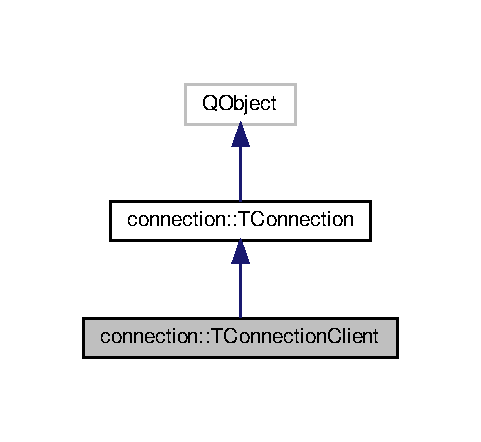
\includegraphics[width=231pt]{classconnection_1_1_t_connection_client__inherit__graph}
\end{center}
\end{figure}


Collaboration diagram for connection\+:\+:T\+Connection\+Client\+:\nopagebreak
\begin{figure}[H]
\begin{center}
\leavevmode
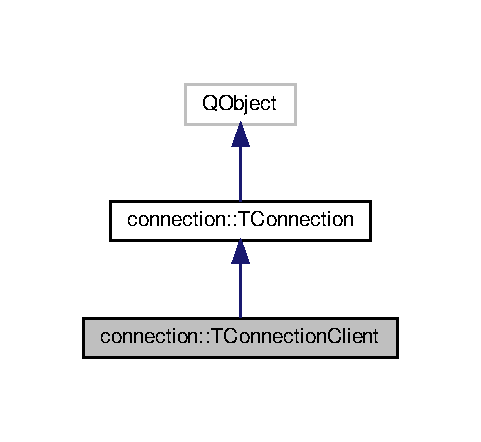
\includegraphics[width=231pt]{classconnection_1_1_t_connection_client__coll__graph}
\end{center}
\end{figure}
\subsection*{Public Member Functions}
\begin{DoxyCompactItemize}
\item 
\mbox{\Hypertarget{classconnection_1_1_t_connection_client_a7aa7cdc07cac6d969ec27518baad8b33}\label{classconnection_1_1_t_connection_client_a7aa7cdc07cac6d969ec27518baad8b33}} 
void {\bfseries seach\+Server} (quint16)
\item 
Q\+Host\+Address \hyperlink{classconnection_1_1_t_connection_client_a00738647cc6afff4d98185faa375ddb4}{get\+Ip\+Address\+Server} ()
\begin{DoxyCompactList}\small\item\em \hyperlink{classconnection_1_1_t_connection_client_a00738647cc6afff4d98185faa375ddb4}{T\+Connection\+Client\+::get\+Ip\+Address\+Server} Получаем адрес найденного сервера \end{DoxyCompactList}\item 
\mbox{\Hypertarget{classconnection_1_1_t_connection_client_a3b902734ae0765b81906eaf987534969}\label{classconnection_1_1_t_connection_client_a3b902734ae0765b81906eaf987534969}} 
bool {\bfseries send\+Data} (\hyperlink{classconnection_1_1_t_connection_a3550181cb2fa72eccfa55d23f45cea34}{T\+Connection\+::exchange\+Protocol}, quint64)
\item 
\mbox{\Hypertarget{classconnection_1_1_t_connection_client_aa4945db8ce32628f90b943c413ffacdc}\label{classconnection_1_1_t_connection_client_aa4945db8ce32628f90b943c413ffacdc}} 
bool {\bfseries receive\+Data} (\hyperlink{classconnection_1_1_t_connection_a3550181cb2fa72eccfa55d23f45cea34}{T\+Connection\+::exchange\+Protocol} $\ast$, quint64 $\ast$)
\end{DoxyCompactItemize}
\subsection*{Additional Inherited Members}


\subsection{Detailed Description}
Класс для работы с сервером раздающим блоки ключей для подбора 

\subsection{Member Function Documentation}
\mbox{\Hypertarget{classconnection_1_1_t_connection_client_a00738647cc6afff4d98185faa375ddb4}\label{classconnection_1_1_t_connection_client_a00738647cc6afff4d98185faa375ddb4}} 
\index{connection\+::\+T\+Connection\+Client@{connection\+::\+T\+Connection\+Client}!get\+Ip\+Address\+Server@{get\+Ip\+Address\+Server}}
\index{get\+Ip\+Address\+Server@{get\+Ip\+Address\+Server}!connection\+::\+T\+Connection\+Client@{connection\+::\+T\+Connection\+Client}}
\subsubsection{\texorpdfstring{get\+Ip\+Address\+Server()}{getIpAddressServer()}}
{\footnotesize\ttfamily Q\+Host\+Address connection\+::\+T\+Connection\+Client\+::get\+Ip\+Address\+Server (\begin{DoxyParamCaption}{ }\end{DoxyParamCaption})}



\hyperlink{classconnection_1_1_t_connection_client_a00738647cc6afff4d98185faa375ddb4}{T\+Connection\+Client\+::get\+Ip\+Address\+Server} Получаем адрес найденного сервера 

\begin{DoxyReturn}{Returns}
Данные найденного сервера 
\end{DoxyReturn}


The documentation for this class was generated from the following files\+:\begin{DoxyCompactItemize}
\item 
client/pr\+S63\+Brute\+Force\+Client/T\+Connection\+Client.\+hpp\item 
client/pr\+S63\+Brute\+Force\+Client/T\+Connection\+Client.\+cpp\end{DoxyCompactItemize}

\hypertarget{classconnection_1_1_t_connection_server}{}\section{connection\+:\+:T\+Connection\+Server Class Reference}
\label{classconnection_1_1_t_connection_server}\index{connection\+::\+T\+Connection\+Server@{connection\+::\+T\+Connection\+Server}}


The \hyperlink{classconnection_1_1_t_connection_server}{T\+Connection\+Server} class Класс для работы с распределённой системой подбора ключей  




{\ttfamily \#include $<$T\+Connection\+Server.\+hpp$>$}



Inheritance diagram for connection\+:\+:T\+Connection\+Server\+:\nopagebreak
\begin{figure}[H]
\begin{center}
\leavevmode
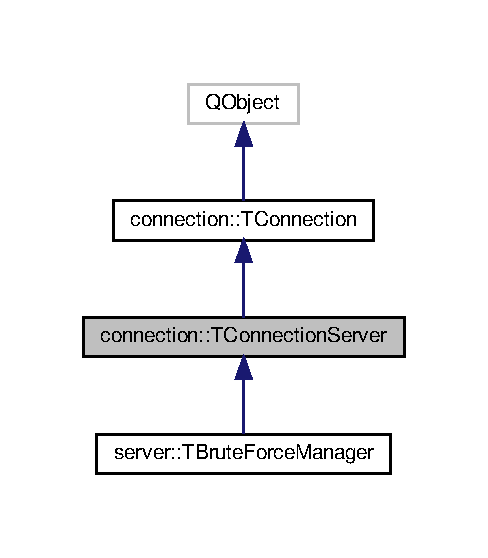
\includegraphics[width=234pt]{classconnection_1_1_t_connection_server__inherit__graph}
\end{center}
\end{figure}


Collaboration diagram for connection\+:\+:T\+Connection\+Server\+:\nopagebreak
\begin{figure}[H]
\begin{center}
\leavevmode
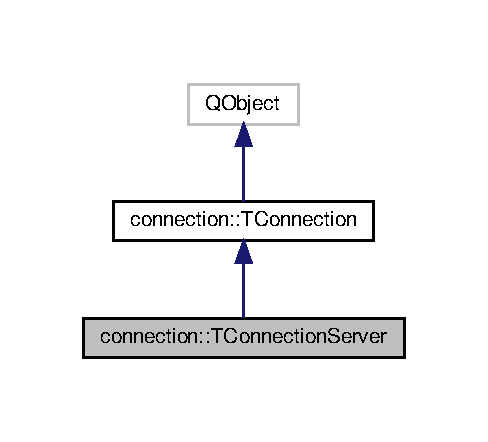
\includegraphics[width=234pt]{classconnection_1_1_t_connection_server__coll__graph}
\end{center}
\end{figure}
\subsection*{Public Member Functions}
\begin{DoxyCompactItemize}
\item 
\mbox{\Hypertarget{classconnection_1_1_t_connection_server_a606ed5e1fd8c97a795abe9e54be5bdeb}\label{classconnection_1_1_t_connection_server_a606ed5e1fd8c97a795abe9e54be5bdeb}} 
\hyperlink{classconnection_1_1_t_connection_server_a606ed5e1fd8c97a795abe9e54be5bdeb}{T\+Connection\+Server} ()
\begin{DoxyCompactList}\small\item\em \hyperlink{classconnection_1_1_t_connection_server_a606ed5e1fd8c97a795abe9e54be5bdeb}{connection\+::\+T\+Connection\+Server\+::\+T\+Connection\+Server} Конструктор \end{DoxyCompactList}\item 
\mbox{\Hypertarget{classconnection_1_1_t_connection_server_a481b658bc12f7bb0b5fee3ccef2937ff}\label{classconnection_1_1_t_connection_server_a481b658bc12f7bb0b5fee3ccef2937ff}} 
bool {\bfseries send\+Data} (\hyperlink{classconnection_1_1_t_connection_a3550181cb2fa72eccfa55d23f45cea34}{T\+Connection\+::exchange\+Protocol}, quint64)
\item 
\mbox{\Hypertarget{classconnection_1_1_t_connection_server_a40b7cdfa826bf501fdb165e965511736}\label{classconnection_1_1_t_connection_server_a40b7cdfa826bf501fdb165e965511736}} 
bool {\bfseries receive\+Data} (\hyperlink{classconnection_1_1_t_connection_a3550181cb2fa72eccfa55d23f45cea34}{T\+Connection\+::exchange\+Protocol} $\ast$, quint64 $\ast$)
\end{DoxyCompactItemize}
\subsection*{Additional Inherited Members}


\subsection{Detailed Description}
The \hyperlink{classconnection_1_1_t_connection_server}{T\+Connection\+Server} class Класс для работы с распределённой системой подбора ключей 

The documentation for this class was generated from the following files\+:\begin{DoxyCompactItemize}
\item 
server/pr\+S63\+Brute\+Force\+Server/T\+Connection\+Server.\+hpp\item 
server/pr\+S63\+Brute\+Force\+Server/T\+Connection\+Server.\+cpp\end{DoxyCompactItemize}

\hypertarget{structcommon_define_client_1_1_t_log_item_client}{}\section{common\+Define\+Client\+:\+:T\+Log\+Item\+Client Struct Reference}
\label{structcommon_define_client_1_1_t_log_item_client}\index{common\+Define\+Client\+::\+T\+Log\+Item\+Client@{common\+Define\+Client\+::\+T\+Log\+Item\+Client}}
\subsection*{Public Attributes}
\begin{DoxyCompactItemize}
\item 
\mbox{\Hypertarget{structcommon_define_client_1_1_t_log_item_client_ab2a6064d43c8dbe637188b3c9b7835a9}\label{structcommon_define_client_1_1_t_log_item_client_ab2a6064d43c8dbe637188b3c9b7835a9}} 
Q\+Time {\bfseries time\+Receive\+Block}
\item 
\mbox{\Hypertarget{structcommon_define_client_1_1_t_log_item_client_aa8d3e11c4173fcd797ce8e8c53d93c8b}\label{structcommon_define_client_1_1_t_log_item_client_aa8d3e11c4173fcd797ce8e8c53d93c8b}} 
quint64 {\bfseries key\+First} \{0\}
\item 
\mbox{\Hypertarget{structcommon_define_client_1_1_t_log_item_client_abe6f35c52279fda23abce2af8ba3da9c}\label{structcommon_define_client_1_1_t_log_item_client_abe6f35c52279fda23abce2af8ba3da9c}} 
std\+::array$<$ quint64, max\+Threads $>$ {\bfseries keys} \{0\}
\item 
\mbox{\Hypertarget{structcommon_define_client_1_1_t_log_item_client_a39a08024bb4f93474f739c4e2636fbe8}\label{structcommon_define_client_1_1_t_log_item_client_a39a08024bb4f93474f739c4e2636fbe8}} 
Q\+Time {\bfseries time\+Send\+Result}
\item 
\mbox{\Hypertarget{structcommon_define_client_1_1_t_log_item_client_a237d46da9198f1a7ad87554186f17f20}\label{structcommon_define_client_1_1_t_log_item_client_a237d46da9198f1a7ad87554186f17f20}} 
Q\+String {\bfseries result} \{\char`\"{}\char`\"{}\}
\end{DoxyCompactItemize}


The documentation for this struct was generated from the following file\+:\begin{DoxyCompactItemize}
\item 
client/pr\+S63\+Brute\+Force\+Client/T\+Common\+Defane\+Client.\+hpp\end{DoxyCompactItemize}

%--- End generated contents ---

% Index
\backmatter
\newpage
\phantomsection
\clearemptydoublepage
\addcontentsline{toc}{chapter}{Index}
\printindex

\end{document}
